% =============================================================================
%  Rapport de Projet de Fin d'Etudes - GRC AI Analyzer
%  Page de garde : modele ENSEM 2019-2020
%  Compilation : pdflatex rapport_pfe.tex (x3 pour TOC + references)
% =============================================================================

\documentclass[a4paper,12pt,oneside]{report}

% --------------------- Encodage et langue ---------------------
\usepackage[utf8]{inputenc}
\usepackage[T1]{fontenc}
\usepackage{lmodern}
\usepackage[french]{babel}

% --------------------- Mise en page ---------------------
\usepackage[a4paper,top=2.5cm,bottom=2.5cm,left=2.5cm,right=2.5cm]{geometry}
\usepackage{setspace}
\onehalfspacing
\setlength{\parindent}{1.5em}
\setlength{\parskip}{6pt}

% --------------------- Maths et symboles ---------------------
\usepackage{amsmath}
\usepackage{amssymb}

% --------------------- Couleurs (theme sobre) ---------------------
\usepackage[table]{xcolor}
\definecolor{darknavy}{RGB}{30,50,90}
\definecolor{titleblue}{RGB}{40,60,110}
\definecolor{lightgray}{RGB}{235,235,235}
\definecolor{boxgray}{RGB}{248,248,248}
\definecolor{darkgreen}{RGB}{30,90,50}

% --------------------- Tableaux ---------------------
\usepackage{array}
\usepackage{booktabs}
\usepackage{multirow}
\usepackage{tabularx}

% --------------------- Flottants ---------------------
\usepackage{float}

% --------------------- Graphiques ---------------------
\usepackage{graphicx}
\usepackage{tikz}
\usetikzlibrary{shapes.geometric,arrows.meta,positioning,fit,calc,backgrounds}
\usepackage{pgfplots}
\pgfplotsset{compat=1.18}
\usetikzlibrary{shapes.arrows, shapes.misc}

% --------------------- Listes ---------------------
\usepackage{enumitem}

% --------------------- Boites et encadres ---------------------
\usepackage[most]{tcolorbox}
\tcbset{
  problemboxstyle/.style={
    colback=boxgray,colframe=darknavy,
    arc=1pt,boxrule=0.5pt,
    left=10pt,right=10pt,top=8pt,bottom=8pt,
    fontupper=\itshape
  },
  critiquestyle/.style={
    colback=boxgray,colframe=darknavy,
    arc=1pt,boxrule=0.5pt,
    left=10pt,right=10pt,top=6pt,bottom=6pt
  },
  infobox/.style={
    colback=boxgray,colframe=darknavy,
    arc=1pt,boxrule=0.3pt,
    left=8pt,right=8pt,top=6pt,bottom=6pt
  }
}

% --------------------- Code source ---------------------
\usepackage{listings}
\lstdefinestyle{pythonstyle}{
  language=Python,
  basicstyle=\ttfamily\footnotesize,
  keywordstyle=\color{darknavy}\bfseries,
  stringstyle=\color{darkgreen},
  commentstyle=\color{gray}\itshape,
  numbers=left,
  numberstyle=\tiny\color{gray},
  backgroundcolor=\color{boxgray},
  frame=single,
  rulecolor=\color{gray!50},
  breaklines=true,
  showstringspaces=false,
  tabsize=2,
  captionpos=b
}
\lstset{style=pythonstyle}

% --------------------- Titres et chapitres ---------------------
\usepackage{titlesec}

\titleformat{\chapter}[hang]
  {\normalfont\Huge\bfseries\color{titleblue}}
  {\thechapter.}{0.8em}{}
\titlespacing*{\chapter}{0pt}{-20pt}{20pt}

\titleformat{\section}
  {\normalfont\Large\bfseries\color{titleblue}}{\thesection}{1em}{}
\titleformat{\subsection}
  {\normalfont\large\bfseries\color{titleblue!85}}{\thesubsection}{1em}{}
\titleformat{\subsubsection}
  {\normalfont\normalsize\bfseries\color{titleblue!70}}{\thesubsubsection}{1em}{}

% --------------------- En-tete / pied de page ---------------------
\usepackage{fancyhdr}
\pagestyle{fancy}
\fancyhf{}
\fancyhead[L]{\textit{\small GRC AI Analyzer}}
\fancyhead[R]{\textit{\small Rapport PFE}}
\fancyfoot[C]{\thepage}
\renewcommand{\headrulewidth}{0.4pt}
\renewcommand{\footrulewidth}{0pt}

\fancypagestyle{plain}{
  \fancyhf{}
  \fancyfoot[C]{\thepage}
  \renewcommand{\headrulewidth}{0pt}
  \renewcommand{\footrulewidth}{0pt}
}

% --------------------- Liens ---------------------
\usepackage[colorlinks=true,linkcolor=darknavy,urlcolor=darknavy,citecolor=darknavy]{hyperref}
\usepackage{url}

% =============================================================================
\begin{document}

% =============================================================================
%  PAGE DE GARDE (modele ENSEM)
% =============================================================================
\begin{titlepage}
\thispagestyle{empty}

% --- Bandeau d'en-tete ---
\noindent\rule{\textwidth}{1.5pt}
\begin{center}
{\small\bfseries Royaume du Maroc \quad $\bullet$ \quad Universit\'e Hassan II de Casablanca}\\
{\small\bfseries \'Ecole Nationale Sup\'erieure d'\'Electricit\'e et de M\'ecanique -- ENSEM}
\end{center}
\noindent\rule{\textwidth}{0.5pt}

\vspace{0.4cm}

% --- Departement et Filiere ---
{\bfseries\large
D\'epartement~: G\'enie Informatique\\[0.3em]
Fili\`ere\hspace{1.4em}: G\'enie Logiciel et Intelligence Artificielle
}

\vspace{1cm}

% --- Logos universite / ecole (placeholders) ---
\begin{center}
\begin{tabular}{cc}
\fbox{\parbox{6cm}{\centering\vspace{2cm}\Large\itshape Logo\\Universit\'e Hassan II\vspace{2cm}}}
&
\fbox{\parbox{6cm}{\centering\vspace{2cm}\Large\itshape Logo\\ENSEM\vspace{2cm}}}
\\
\end{tabular}
\end{center}

\vspace{1cm}

% --- Titre principal ---
\begin{center}
{\Huge\bfseries\itshape\color{titleblue} RAPPORT DE PROJET\\[0.3em] DE FIN D'\'ETUDES}
\end{center}

\vspace{0.8cm}

% --- Societe ---
\begin{center}
{\large\itshape R\'ealis\'e au sein de} {\large\bfseries\itshape [Nom de la Soci\'et\'e]}

\vspace{0.6cm}

\fbox{\parbox{6cm}{\centering\vspace{1.5cm}\Large\itshape Logo Soci\'et\'e\vspace{1.5cm}}}
\end{center}

\vspace{0.8cm}

% --- Theme ---
{\bfseries\large TH\`EME~:}

\begin{center}
\vspace{0.4cm}
\fbox{\parbox{0.9\textwidth}{\centering\vspace{0.3cm}
{\LARGE\bfseries\color{titleblue} GRC AI Analyzer}\\[0.4em]
{\large Plateforme d'analyse automatis\'ee des rapports\\ de gouvernance, risque et conformit\'e\\ propuls\'ee par l'Intelligence Artificielle G\'en\'erative}
\vspace{0.3cm}}}
\end{center}

\vspace{1cm}

% --- Jury / encadrants ---
\renewcommand{\arraystretch}{1.5}
\noindent\begin{tabular}{p{8cm}p{7cm}}
\bfseries Soutenu le~~\rule{0.6cm}{0.4pt}~-~\rule{0.6cm}{0.4pt}~-~2026 par~: & \bfseries Encadr\'e par~: \\
\quad -- Mahdi BOUKHOUALI & \quad -- Prof.~[Nom Pr\'enom] (Encadrant ENSEM) \\
 & \quad -- M.~[Nom Pr\'enom] (Encadrant Industriel) \\[0.4em]
\bfseries Devant les membres du jury~: & \\
\quad -- Pr.~[Nom Pr\'enom] \hfill Pr\'esident & \\
\quad -- Pr.~[Nom Pr\'enom] \hfill Rapporteur & \\
\quad -- Pr.~[Nom Pr\'enom] \hfill Encadrant ENSEM & \\
\quad -- M.~[Nom Pr\'enom] \hfill Encadrant Industriel & \\
\end{tabular}

\vfill

\hfill{\bfseries\large Promotion 2026}

\end{titlepage}

% =============================================================================
%  PAGES PRELIMINAIRES
% =============================================================================
\pagenumbering{Roman}

% --- Dedicace ---
\chapter*{D\'edicace}
\addcontentsline{toc}{chapter}{D\'edicace}
\thispagestyle{plain}

\begin{quote}\itshape
C'est avec une profonde gratitude et une immense fiert\'e que je d\'edie ce modeste travail, fruit de plusieurs mois d'efforts et de recherche, aux personnes qui ont marqu\'e mon parcours acad\'emique et personnel.

\medskip
Je d\'edie ce rapport en premier lieu \`a ma famille, et plus particuli\`erement \`a mes chers parents, qui ont toujours \'et\'e ma source d'inspiration et le pilier de ma r\'eussite. Aucun mot ne saurait exprimer l'ampleur de ma reconnaissance pour leurs innombrables sacrifices, leur soutien inconditionnel et leurs pri\`eres qui m'ont accompagn\'e dans chaque \'etape.

\medskip
\`A mes fr\`eres et s{\oe}urs, pour leur pr\'esence r\'econfortante et leur belle complicit\'e. Que ce travail soit l'humble t\'emoignage de mon affection et de ma gratitude \'eternelle.

\medskip
Je d\'edie \'egalement ce projet \`a mes encadrants, dont l'orientation rigoureuse, la disponibilit\'e et les pr\'ecieux conseils ont \'et\'e une v\'eritable boussole tout au long de ce stage de fin d'\'etudes.

\medskip
Enfin, je souhaite d\'edier ce travail \`a tous mes amis, coll\`egues et professeurs de l'\'ecole, qui ont contribu\'e, de pr\`es ou de loin, \`a mon \'evolution et \`a l'aboutissement de ce projet.
\end{quote}

% --- Remerciements ---
\chapter*{Remerciements}
\addcontentsline{toc}{chapter}{Remerciements}
\thispagestyle{plain}

Je tiens \`a exprimer ma plus sinc\`ere gratitude \`a l'ensemble des personnes qui ont contribu\'e \`a la r\'ealisation de ce travail, tant sur le plan acad\'emique que professionnel et personnel.

Tout d'abord, je remercie chaleureusement mes parents pour leur amour inconditionnel, leur patience in\'epuisable et leur soutien ind\'efectible tout au long de mon parcours. Leur confiance en moi et leurs encouragements constants ont \'et\'e le pilier de ma r\'eussite.

Je tiens \'egalement \`a exprimer toute ma reconnaissance \`a mon encadrant p\'edagogique, Prof.~[Nom de l'encadrant acad\'emique], pour sa disponibilit\'e, ses conseils judicieux et son accompagnement rigoureux. Son regard critique et ses orientations m\'ethodologiques ont grandement contribu\'e \`a la qualit\'e de ce projet.

Mes remerciements vont \'egalement \`a mon encadrant professionnel, M.~[Nom de l'encadrant industriel], pour sa confiance, son suivi attentif et son partage d'expertise dans le domaine de la gouvernance, du risque et de la conformit\'e. Sa vision technique et m\'etier a grandement enrichi ce travail.

Je remercie aussi l'ensemble de l'\'equipe avec laquelle j'ai eu le privil\`ege de collaborer durant cette p\'eriode. Les \'echanges enrichissants et l'esprit collaboratif ont fait de cette exp\'erience une aventure humaine et professionnelle inoubliable.

Enfin, j'adresse mes remerciements \`a l'ensemble du corps professoral de l'ENSEM, ainsi qu'\`a mes camarades de promotion, pour les ann\'ees de formation qui ont rendu possible ce projet.

% --- Resume ---
\chapter*{R\'esum\'e}
\addcontentsline{toc}{chapter}{R\'esum\'e}
\thispagestyle{plain}

Dans un contexte mondial marqu\'e par la multiplication des r\'eglementations en mati\`ere de protection des donn\'ees et de cybers\'ecurit\'e, les organisations sont confront\'ees \`a une charge croissante d'analyse de leurs rapports de gouvernance, de risque et de conformit\'e (GRC). L'analyse manuelle de ces documents est chronophage, sujette aux erreurs et difficilement scalable.

C'est dans ce cadre que s'inscrit ce projet de fin d'\'etudes, dont l'objectif est la conception et la r\'ealisation de \textbf{GRC AI Analyzer}, une plateforme \emph{full-stack} d'analyse automatis\'ee des rapports GRC propuls\'ee par l'intelligence artificielle g\'en\'erative. Le syst\`eme permet l'import de documents aux formats PDF, DOCX et XLSX, puis exploite le mod\`ele \textbf{Mistral AI} pour extraire automatiquement les risques, \'evaluer la conformit\'e vis-\`a-vis des r\'ef\'erentiels \textbf{ISO~27001}, \textbf{RGPD} et de la \textbf{Loi 09-08} marocaine, et g\'en\'erer des recommandations concr\`etes.

L'architecture repose sur un backend \textbf{FastAPI} asynchrone, une persistance \textbf{PostgreSQL}, un stockage objet \textbf{MinIO}, une base vectorielle \textbf{ChromaDB} pour le \emph{Retrieval Augmented Generation} (RAG), et une interface utilisateur \textbf{React/Vite} moderne. Un pipeline d'analyse en deux phases parall\`eles assure des temps de traitement r\'eduits, tandis qu'une interface conversationnelle bas\'ee sur le RAG permet \`a l'utilisateur d'interroger directement le rapport analys\'e.

\medskip
\textbf{Mots-cl\'es :} GRC, Intelligence Artificielle, Mistral, RAG, ChromaDB, FastAPI, React, ISO~27001, RGPD, Loi 09-08, conformit\'e, gestion des risques.

% --- Abstract ---
\chapter*{Abstract}
\addcontentsline{toc}{chapter}{Abstract}
\thispagestyle{plain}

In a global context marked by the multiplication of regulations regarding data protection and cybersecurity, organizations face a growing burden in analyzing their Governance, Risk and Compliance (GRC) reports. Manual analysis of these documents is time-consuming, error-prone and hardly scalable.

This end-of-studies project introduces \textbf{GRC AI Analyzer}, a full-stack platform for automated GRC report analysis powered by generative artificial intelligence. The system enables document upload in PDF, DOCX and XLSX formats, then leverages the \textbf{Mistral AI} model to automatically extract risks, evaluate compliance against \textbf{ISO~27001}, \textbf{GDPR} and Morocco's \textbf{Law 09-08}, and generate concrete recommendations.

The architecture relies on an asynchronous \textbf{FastAPI} backend, a \textbf{PostgreSQL} database, a \textbf{MinIO} object store, a \textbf{ChromaDB} vector database for Retrieval Augmented Generation (RAG), and a modern \textbf{React/Vite} user interface. A two-phase parallel analysis pipeline ensures reduced processing times, while a conversational interface based on RAG allows users to directly interrogate analyzed reports.

\medskip
\textbf{Keywords:} GRC, Artificial Intelligence, Mistral, RAG, ChromaDB, FastAPI, React, ISO~27001, GDPR, Law 09-08, compliance, risk management.

% --- TOC, LOF, LOT ---
\renewcommand{\contentsname}{Table des mati\`eres}
\tableofcontents
\listoffigures
\listoftables

\chapter*{Liste des acronymes}
\addcontentsline{toc}{chapter}{Liste des acronymes}

\begin{description}[leftmargin=2.5cm,style=nextline,itemsep=2pt]
  \item[\textbf{API}] Application Programming Interface
  \item[\textbf{CRUD}] Create, Read, Update, Delete
  \item[\textbf{DTO}] Data Transfer Object
  \item[\textbf{GRC}] Governance, Risk and Compliance
  \item[\textbf{ISO}] International Organization for Standardization
  \item[\textbf{JWT}] JSON Web Token
  \item[\textbf{LLM}] Large Language Model
  \item[\textbf{ORM}] Object Relational Mapping
  \item[\textbf{PDF}] Portable Document Format
  \item[\textbf{PFE}] Projet de Fin d'\'Etudes
  \item[\textbf{RAG}] Retrieval Augmented Generation
  \item[\textbf{REST}] Representational State Transfer
  \item[\textbf{RGPD}] R\`eglement G\'en\'eral sur la Protection des Donn\'ees
  \item[\textbf{SPA}] Single Page Application
  \item[\textbf{SQL}] Structured Query Language
  \item[\textbf{UI}] User Interface
  \item[\textbf{UX}] User Experience
\end{description}

% =============================================================================
\clearpage
\pagenumbering{arabic}
% =============================================================================

% =============================================================================
%  CHAPITRE 1
% =============================================================================
\chapter{Pr\'esentation du cadre du projet}


\section{Introduction}
Ce premier chapitre a pour objectif de placer le projet dans son environnement professionnel, m\'etier et r\'eglementaire. Avant d'aborder l'analyse d\'etaill\'ee des besoins et la conception de la solution, il est n\'ecessaire de comprendre le contexte dans lequel s'inscrit la cr\'eation de \emph{GRC AI Analyzer}, une plateforme d'analyse automatis\'ee des rapports de gouvernance, risque et conformit\'e propuls\'ee par l'intelligence artificielle.

Le chapitre pr\'esente d'abord l'organisme d'accueil, ainsi que le contexte m\'etier de la GRC. Il expose ensuite les enjeux r\'eglementaires (ISO~27001, RGPD, Loi 09-08), analyse les limites des approches manuelles existantes, formule la probl\'ematique du projet et pr\'esente la solution envisag\'ee.

% =============================================================================
%  SECTION 1 — PRÉSENTATION DE L'ORGANISME D'ACCUEIL
% =============================================================================
\section{Pr\'esentation de l'organisme d'accueil}

\subsection{Pr\'esentation g\'en\'erale}
Evolvity Partners est un cabinet marocain de conseil sp\'ecialis\'e en cybers\'ecurit\'e et en gestion des risques, fond\'e en 2022. S'appuyant sur un pool d'experts capitalisant plus de douze ann\'ees d'exp\'erience cumul\'ee, la structure a connu une croissance rapide~: deux consultants \`a sa cr\'eation, quatre en 2024, dix en 2025, avec une projection d'expansion internationale \`a l'horizon 2027. Ses locaux accueillent aujourd'hui une \'equipe pluridisciplinaire d\'edi\'ee \`a accompagner ses clients au Maroc et \`a l'international, selon une approche sur mesure conforme aux standards internationaux les plus exigeants. 
\subsection{Domaines d'expertise et offre de services}

L'offre d'Evolvity Partners est structur\'ee autour de quatre p\^oles compl\'ementaires couvrant l'ensemble du spectre de la cybers\'ecurit\'e.

\begin{itemize}
	\item \textbf{Audit~:} Le p\^ole Audit d\'eploie des missions d'\'evaluation \`a plusieurs niveaux~:Organisationnel, Technique et Physique.
	\item \textbf{GRC~:} Le p\^ole GRC constitue le c\oe ur strat\'egique de l'activit\'e et couvre~:
	\item \textbf{Technologie~:} Le p\^ole Technologie couvre les domaines \'emergents~: Cloud, Blockchain, IoT et OT, avec une capacit\'e d'int\'egration de solutions s\'ecuris\'ees dans des environnements complexes et h\'et\'erog\`enes.
	\item \textbf{ISS As A Service~:} Ce mod\`ele de prestation externalis\'ee met \`a disposition des clients des profils sp\'ecialis\'es en mode r\'egie ou forfait~: RSSI (\textit{Responsable de la S\'ecurit\'e des Syst\`emes d'Information}), SecOps, PMO et experts m\'etier, offrant ainsi une flexibilit\'e adapt\'ee aux organisations ne disposant pas de ces comp\'etences en interne.
	
\end{itemize}

\begin{figure}[ht]
	\centering
	\begin{tikzpicture}[node distance=1.2cm and 1.5cm]
		\tikzstyle{actbox}=[rectangle,draw=darknavy,thick,fill=lightgray,
		minimum width=3.2cm,minimum height=1cm,
		rounded corners=2pt,align=center,font=\small]
		\node[actbox] (audit)  {Audit\\(Org./Tech./Phys.)};
		\node[actbox,right=of audit]  (grc)   {GRC\\(Gov./Risque/Conf.)};
		\node[actbox,right=of grc]    (tech)  {Technologie\\(Cloud/IoT/OT)};
		\node[actbox,right=of tech]   (iss)   {ISS As A\\Service};
		\node[actbox,below=2cm of grc,xshift=1.85cm,
		minimum width=7cm,fill=darknavy!15,draw=darknavy,font=\small\bfseries]
		(core) {Cybers\'ecurit\'e \& Conformit\'e r\'eglementaire};
		\draw[-{Latex[length=2mm]},darknavy] (audit) -- (core);
		\draw[-{Latex[length=2mm]},darknavy] (grc)   -- (core);
		\draw[-{Latex[length=2mm]},darknavy] (tech)  -- (core);
		\draw[-{Latex[length=2mm]},darknavy] (iss)   -- (core);
	\end{tikzpicture}
	\caption{Les quatre p\^oles de l'offre Evolvity Partners}
	\label{fig:activites}
\end{figure}

\subsection{Positionnement et client\`ele}

Evolvity Partners s'adresse principalement aux banques, institutions financi\`eres, administrations publiques et grandes entreprises op\'erant dans des secteurs r\'eglement\'es. Son positionnement repose sur une approche qui allie rigueur technique, conformit\'e r\'eglementaire et gestion des risques strat\'egiques, avec pour objectif de prot\'eger les actifs num\'eriques de ses clients tout en accompagnant leur transformation digitale.

\subsection{Cadre du projet GRC AI Analyzer}

Le projet \textit{GRC AI Analyzer}, objet du pr\'esent rapport, s'inscrit directement dans le p\^ole GRC d'Evolvity Partners. Face au volume croissant de rapports d'audit, de politiques de s\'ecurit\'e et de documents de conformit\'e trait\'es par les consultants, l'entreprise a identifi\'e un besoin strat\'egique d'automatisation de l'analyse documentaire. Le projet vise \`a industrialiser cette pratique gr\^ace \`a une plateforme propuls\'ee par l'intelligence artificielle g\'en\'erative, r\'eduisant ainsi les d\'elais d'analyse et augmentant la pr\'ecision des diagnostics de conformit\'e.
```

\section{Contexte m\'etier : la Gouvernance, le Risque et la Conformit\'e (GRC)}

La GRC (\textit{Governance, Risk and Compliance}) d\'esigne le cadre int\'egr\'e par lequel une organisation structure et coordonne ses pratiques de gouvernance, de gestion des risques et de conformit\'e r\'eglementaire. Loin d'être trois disciplines ind\'ependantes, ces trois dimensions forment un syst\`eme coh\'erent~: une gouvernance solide oriente la gestion des risques, qui elle-m\^eme conditionne la capacit\'e de l'organisation \`a satisfaire ses obligations de conformit\'e. Dans un contexte o\`u les cybermenaces se multiplient et o\`u les exigences r\'eglementaires s'intensifient, la GRC est devenue un levier strat\'egique indispensable pour toute organisation souhaitant ma\^itriser son exposition et pr\'eserver la confiance de ses parties prenantes.

\subsection{Les trois piliers de la GRC}

\subsubsection*{Gouvernance}
La gouvernance d\'esigne l'ensemble des m\'ecanismes par lesquels une organisation d\'efinit ses orientations strat\'egiques, r\'epartit les responsabilit\'es et s'assure que ses d\'ecisions sont align\'ees avec ses objectifs. En mati\`ere de s\'ecurit\'e de l'information, la gouvernance se traduit concr\`etement par~:
\begin{itemize}[leftmargin=1.5em,itemsep=2pt]
	\item l'\'elaboration de politiques de s\'ecurit\'e et de chartes d'utilisation des syst\`emes d'information~;
	\item la d\'efinition de structures organisationnelles claires (RSSI, DPO, comit\'es de s\'ecurit\'e)~;
	\item la mise en place d'indicateurs de pilotage (KPI, tableaux de bord) permettant un suivi continu de la maturit\'e s\'ecurit\'e~;
	\item la conduite de programmes de sensibilisation et de formation des collaborateurs.
\end{itemize}
Une gouvernance efficace constitue le socle sur lequel reposent les deux autres piliers~: sans cadre d\'ecisionnel clair, ni la gestion des risques ni la conformit\'e ne peuvent \^etre men\'ees de mani\`ere coh\'erente.

\subsubsection*{Gestion des risques}
La gestion des risques vise \`a identifier, analyser, \'evaluer et traiter les menaces susceptibles d'affecter les actifs strat\'egiques d'une organisation. Elle s'articule autour d'un processus it\'eratif~:
\begin{enumerate}[leftmargin=1.5em,itemsep=2pt]
	\item \textbf{Identification~:} recensement des actifs (donn\'ees, syst\`emes, processus) et des menaces associ\'ees~;
	\item \textbf{Analyse~:} \'evaluation de la probabilit\'e et de l'impact de chaque sc\'enario de risque~;
	\item \textbf{\'Evaluation~:} priorisation des risques selon leur niveau de criticit\'e~;
	\item \textbf{Traitement~:} choix d'une strat\'egie parmi l'acceptation, la r\'eduction, le transfert ou l'\'evitement du risque~;
	\item \textbf{Suivi~:} surveillance continue et r\'e\'evaluation p\'eriodique.
\end{enumerate}
Les m\'ethodologies de r\'ef\'erence utilis\'ees dans ce domaine incluent notamment ISO~31000 (management du risque), ISO~27005 (gestion des risques li\'es \`a la s\'ecurit\'e de l'information) et EBIOS Risk Manager (m\'ethode fran\c{c}aise d'analyse des risques num\'eriques).

\subsubsection*{Conformit\'e}
La conformit\'e d\'esigne le respect des obligations l\'egales, r\'eglementaires, normatives et contractuelles applicables \`a l'organisation. Elle implique~:
\begin{itemize}[leftmargin=1.5em,itemsep=2pt]
	\item une veille r\'eglementaire permanente pour identifier les textes applicables~;
	\item des audits internes et externes r\'eguliers pour mesurer l'\'ecart entre l'\'etat r\'eel et les exigences~;
	\item la mise en \oe uvre de plans d'actions correctives pour r\'esorber les non-conformit\'es~;
	\item la production de rapports et de preuves documentaires \`a destination des autorit\'es de contr\^ole.
\end{itemize}
La non-conformit\'e expose l'organisation \`a des sanctions financi\`eres, des atteintes \`a sa r\'eputation, voire des interruptions d'activit\'e. C'est pourquoi la conformit\'e ne saurait \^etre trait\'ee comme une contrainte ponctuelle, mais comme un processus continu int\'egr\'e \`a la strat\'egie de l'entreprise.

\subsection{Cadres r\'eglementaires et normatifs retenus}

Dans le cadre du projet GRC AI Analyzer, trois r\'ef\'erentiels ont \'et\'e s\'electionn\'es pour leur pertinence strat\'egique dans le contexte marocain et international, ainsi que pour leur compl\'ementarit\'e dans la couverture des enjeux de s\'ecurit\'e et de protection des donn\'ees.

\begin{table}[ht]
	\centering
	\renewcommand{\arraystretch}{1.4}
	\begin{tabular}{|l|l|l|}
		\hline
		\rowcolor{lightgray}
		\textbf{R\'ef\'erentiel} & \textbf{Domaine} & \textbf{Port\'ee} \\
		\hline
		ISO 27001:2022 & S\'ecurit\'e de l'information & Internationale \\
		\hline
		RGPD & Protection des donn\'ees personnelles & Union Europ\'eenne \\
		\hline
		Loi 09-08 & Protection des donn\'ees personnelles & Royaume du Maroc \\
		\hline
	\end{tabular}
	\caption{R\'ef\'erentiels de conformit\'e couverts par la plateforme}
	\label{tab:referentiels}
\end{table}

\subsubsection*{ISO 27001:2022 --- Syst\`eme de Management de la S\'ecurit\'e de l'Information}
La norme ISO/IEC~27001 est la r\'ef\'erence internationale pour la mise en place, l'exploitation, la surveillance, la maintenance et l'am\'elioration continue d'un Syst\`eme de Management de la S\'ecurit\'e de l'Information (SMSI). Dans sa version 2022, elle s'articule autour de deux composantes principales~:
\begin{itemize}[leftmargin=1.5em,itemsep=2pt]
	\item \textbf{Le corps normatif (clauses 4 \`a 10)~:} il d\'efinit les exigences organisationnelles que tout SMSI doit satisfaire~: contexte de l'organisation, leadership, planification, support, op\'erations, \'evaluation des performances et am\'elioration~;
	\item \textbf{L'annexe A~:} elle regroupe 93~mesures de s\'ecurit\'e (contr\^oles) r\'eparties en quatre cat\'egories~: organisationnelles (37), humaines (8), physiques (14) et technologiques (34).
\end{itemize}
L'obtention de la certification ISO~27001 atteste qu'une organisation a mis en place un SMSI conforme aux meilleures pratiques internationales. Elle est aujourd'hui exig\'ee par de nombreux donneurs d'ordre, notamment dans les secteurs bancaire, assurantiel et des op\'erateurs d'importance vitale. L'analyse automatis\'ee des \'ecarts (\textit{gap analysis}) par rapport aux exigences ISO~27001 constitue l'un des cas d'usage centraux de la plateforme GRC AI Analyzer.

\subsubsection*{RGPD --- R\`eglement G\'en\'eral sur la Protection des Donn\'ees}
Entr\'e en vigueur le 25~mai 2018, le R\`eglement (UE) 2016/679, dit RGPD, est le texte fondateur de la protection des donn\'ees personnelles au sein de l'Union Europ\'eenne. Son champ d'application est extraterritorial~: toute organisation, o\`u qu'elle soit \'etablie, qui traite des donn\'ees de r\'esidents europ\'eens est soumise \`a ses dispositions. Parmi ses principes structurants~:
\begin{itemize}[leftmargin=1.5em,itemsep=2pt]
	\item \textbf{Liceit\'e, loyaut\'e et transparence~:} le traitement doit reposer sur une base l\'egale explicite (consentement, ex\'ecution d'un contrat, obligation l\'egale, etc.)~;
	\item \textbf{Limitation des finalit\'es~:} les donn\'ees collect\'ees ne peuvent \^etre utilis\'ees qu'\`a des fins d\'etermin\'ees et l\'egitimes~;
	\item \textbf{Minimisation des donn\'ees~:} seules les donn\'ees strictement n\'ecessaires doivent \^etre collect\'ees~;
	\item \textbf{Droits des personnes concern\'ees~:} droit d'acc\`es, de rectification, d'effacement, de portabilit\'e et d'opposition~;
	\item \textbf{Responsabilit\'e (\textit{accountability})~:} l'organisation doit \^etre en mesure de d\'emontrer sa conformit\'e \`a tout moment.
\end{itemize}
Les sanctions pr\'evues peuvent atteindre 20~millions d'euros ou 4~\% du chiffre d'affaires mondial annuel. Le DPO (\textit{Data Protection Officer}) joue un r\^ole central dans la supervision de la conformit\'e RGPD au sein des organisations concern\'ees.

\subsubsection*{Loi 09-08 --- Protection des Donn\'ees Personnelles au Maroc}
Promulgu\'ee en 2009 et renforc\'ee par la Loi~31-13 relative au droit d'acc\`es \`a l'information, la Loi~09-08 constitue le cadre l\'egal marocain de protection des donn\'ees \`a caract\`ere personnel. Elle est plac\'ee sous la supervision de la \textbf{CNDP} (Commission Nationale de contr\^ole de la protection des Donn\'ees \`a caract\`ere Personnel). Ses principales dispositions portent sur~:
\begin{itemize}[leftmargin=1.5em,itemsep=2pt]
	\item l'obligation de d\'eclaration ou d'autorisation pr\'ealable de tout traitement de donn\'ees personnelles aupr\`es de la CNDP~;
	\item le respect des droits des personnes concern\'ees~: droit d'information, d'acc\`es, de rectification et d'opposition~;
	\item l'encadrement des transferts de donn\'ees vers des pays tiers~;
	\item des obligations de s\'ecurit\'e et de confidentialit\'e impos\'ees aux responsables de traitement.
\end{itemize}
Si la Loi~09-08 pr\'esente des similitudes structurelles avec le RGPD europ\'een, elle s'en distingue notamment par ses modalit\'es de contr\^ole et l'\'etendue des obligations d\'eclaratives. Dans le contexte des clients marocains d'Evolvity Partners, la double conformit\'e RGPD / Loi~09-08 est fr\'equemment requise, justifiant l'int\'egration simultan\'ee des deux r\'ef\'erentiels dans la plateforme.

\subsection{Enjeux de l'analyse documentaire GRC}

Les cabinets de conseil en GRC produisent et analysent quotidiennement un volume consid\'erable de documents~: politiques de s\'ecurit\'e, rapports d'audit, plans de traitement des risques, preuves de conformit\'e. L'analyse manuelle de ces documents est chronophage, sujette aux erreurs d'interpr\'etation et difficile \`a standardiser entre consultants. C'est pr\'ecis\'ement ce verrou op\'erationnel que le projet GRC AI Analyzer vise \`a lever, en automatisant l'extraction, la structuration et l'\'evaluation des informations pertinentes contenues dans ces documents, au regard des exigences des r\'ef\'erentiels ISO~27001, RGPD et Loi~09-08.

\section{\'Etude de l'existant}

\subsection{Pratiques actuelles d'analyse des rapports GRC}

L'analyse des rapports de gouvernance, risque et conformit\'e est aujourd'hui enti\`erement manuelle au sein des cabinets de conseil. Ce processus mobilise un consultant senior pendant plusieurs jours et se d\'ecompose en six \'etapes s\'equentielles, illustr\'ees dans la figure~\ref{fig:flux_manuel}.

\begin{enumerate}[leftmargin=1.5em,itemsep=4pt]
	\item \textbf{R\'eception du rapport~:} le document est transmis au cabinet sous forme de fichier PDF, Word ou scan. Il peut s'agir d'une politique de s\'ecurit\'e, d'un rapport d'audit interne, d'un registre de traitements ou de tout autre livrable GRC.
	\item \textbf{Lecture int\'egrale par un consultant senior~:} un expert parcourt l'int\'egralit\'e du document afin d'en saisir le contexte, d'identifier les sections pertinentes et de former un premier jugement sur la maturit\'e de l'organisation.
	\item \textbf{Surlignage manuel des passages \`a risque~:} le consultant annote manuellement les passages susceptibles de r\'ev\'eler une non-conformit\'e, une lacune de contr\^ole ou un risque non trait\'e, sans garantie d'exhaustivit\'e ni de coh\'erence inter-consultants.
	\item \textbf{Saisie dans un tableur Excel ou Word~:} les observations relev\'ees sont retranscrites manuellement dans un mod\`ele de rapport structur\'e, op\'eration fastidieuse et source d'erreurs de saisie.
	\item \textbf{Recoupement manuel avec les contr\^oles ISO / RGPD / 09-08~:} chaque observation est mise en correspondance avec les exigences des r\'ef\'erentiels applicables, n\'ecessitant une connaissance approfondie et \`a jour de l'ensemble des contr\^oles concern\'es.
	\item \textbf{R\'edaction du rapport de synth\`ese~:} le consultant produit un rapport final consolid\'e, incluant les \'ecarts identifi\'es, leur niveau de criticit\'e et les recommandations associ\'ees.
\end{enumerate}


Ce processus pr\'esente plusieurs limites op\'erationnelles majeure. C'est l'ensemble de ces frictions que le projet GRC AI Analyzer vise \`a r\'esoudre.

\subsection{Limites des approches existantes}

\begin{figure}[ht]
\centering
\begin{tikzpicture}[node distance=0.4cm]
  \tikzstyle{limit}=[rectangle,draw=darknavy,thick,fill=lightgray,minimum width=10cm,minimum height=0.8cm,rounded corners=2pt,align=center]
  \node[limit] (l1) {\textbf{Temps} : analyse manuelle de 5 \`a 10 jours par rapport};
  \node[limit,below=of l1] (l2) {\textbf{Co\^ut} : mobilisation de consultants seniors};
  \node[limit,below=of l2] (l3) {\textbf{Erreurs} : oubli ou mauvaise interpr\'etation};
  \node[limit,below=of l3] (l4) {\textbf{Subjectivit\'e} : variabilit\'e entre auditeurs};
  \node[limit,below=of l4] (l5) {\textbf{Scalabilit\'e} : difficile sur grands volumes};
\end{tikzpicture}
\caption{Limites identifi\'ees dans les pratiques actuelles}
\label{fig:limites}
\end{figure}

\subsection{Solutions du march\'e et limites de l'existant}

\subsubsection*{Leaders du march\'e GRC}

Les plateformes commerciales dominantes --- RSA Archer, ServiceNow GRC et MetricStream --- offrent des fonctionnalit\'es \'etendues de gestion des risques, des audits et de la conformit\'e. Destin\'ees aux grandes entreprises, elles souffrent n\'eanmoins de limitations communes~: co\^uts de licence prohibitifs, d\'eploiements longs et complexes, et surtout une architecture bas\'ee sur la saisie manuelle de donn\'ees structur\'ees. Aucune ne propose d'analyse automatique de documents non structur\'es, et aucune ne couvre nativement le cadre r\'eglementaire marocain (Loi~09-08).

\subsubsection*{Solutions open-source}

Des outils tels qu'Eramba, SimpleRisk ou OpenGRC proposent des alternatives accessibles pour les organisations \`a budget limit\'e. Ils couvrent les fonctions de base~: registre des risques, suivi des contr\^oles, gestion des audits. Leurs limites sont toutefois significatives~: interfaces rudimentaires, absence de support des r\'ef\'erentiels r\'egionaux, communaut\'es restreintes, et aucune capacit\'e d'analyse s\'emantique ou d'intelligence artificielle int\'egr\'ee.

\subsubsection*{Outils bas\'es sur les LLM}

L'int\'egration des mod\`eles de langage dans le domaine GRC est embryonnaire. Quelques exp\'erimentations existent~: usage de ChatGPT en mode ad hoc pour r\'esumer des politiques, ou plugins Copilot pour l'analyse de documents Office. Ces usages restent non structur\'es, sans ancrage aux r\'ef\'erentiels normatifs, sans tra\c{c}abilit\'e des sources, et inadapt\'es \`a un contexte professionnel d'audit o\`u la pr\'ecision et la justification des \'ecarts sont indispensables.

\begin{tcolorbox}[critiquestyle]
	\textbf{Synth\`ese.} Aucune solution existante ne combine simultan\'ement une analyse automatis\'ee de documents non structur\'es, une couverture multi-r\'ef\'erentiels incluant la Loi~09-08, et une interface conversationnelle ancr\'ee aux normes GRC. Cette lacune justifie la conception de GRC AI Analyzer.
\end{tcolorbox}

\section{Probl\'ematique du projet}

L'analyse des rapports GRC pr\'esente une dualit\'e trompeuse, illustr\'ee par la m\'etaphore de l'iceberg~: ce qui est visible --- le rapport rendu et la conformit\'e d\'eclar\'ee, les recommandations transmises au client --- ne repr\'esente qu'une infime partie du travail r\'eel. La masse immerg\'ee, invisible au commanditaire, concentre l'essentiel de l'effort et des risques~: des dizaines d'heures d'analyse manuelle, d'annotations dispers\'ees et de relectures r\'ep\'et\'ees~; une interpr\'etation des normes qui varie selon l'expert, sans tra\c{c}abilit\'e des choix effectu\'es~; et surtout, des risques non d\'etect\'es et des priorit\'es fix\'ees \`a l'intuition, faute de temps ou de m\'ethode. C'est pr\'ecis\'ement cette partie invisible qui constitue le terreau des non-conformit\'es non identifi\'ees et des recommandations incompl\`etes.

La probl\'ematique centrale peut d\`es lors \^etre formul\'ee comme suit~:

\begin{tcolorbox}[problemboxstyle]
	Comment concevoir une plateforme intelligente capable d'automatiser l'analyse des rapports GRC h\'et\'erog\`enes (PDF, DOCX, XLSX), d'extraire les risques, d'\'evaluer la conformit\'e vis-\`a-vis des r\'ef\'erentiels ISO~27001, RGPD et Loi~09-08, et de fournir une interface conversationnelle exploitant le contenu analys\'e, tout en garantissant performance, fiabilit\'e et s\'ecurit\'e~?
\end{tcolorbox}

\section{Solution envisag\'ee}
La solution propos\'ee, baptis\'ee \textbf{GRC AI Analyzer}, est une plateforme \emph{full-stack} compos\'ee d'un module d'ingestion documentaire prenant en charge PDF, DOCX et XLSX, d'un pipeline d'analyse asynchrone mobilisant le LLM Mistral AI, d'un moteur de Retrieval Augmented Generation pour le chat conversationnel, et d'une interface utilisateur React pour la visualisation et l'export des r\'esultats.

\begin{figure}[ht]
\centering
\begin{tikzpicture}[node distance=1.4cm and 1.6cm]
  \tikzstyle{layer}=[rectangle,draw=darknavy,thick,minimum width=3.5cm,minimum height=1.1cm,rounded corners=3pt,align=center]
  \node[layer,fill=lightgray] (front) {\textbf{Frontend}\\React + Vite};
  \node[layer,fill=lightgray,below=of front] (back) {\textbf{Backend FastAPI}\\Async + JWT};
  \node[layer,fill=boxgray,below left=of back,xshift=-0.5cm] (db) {\textbf{PostgreSQL}\\M\'etadonn\'ees};
  \node[layer,fill=boxgray,below=of back] (minio) {\textbf{MinIO}\\Stockage fichiers};
  \node[layer,fill=boxgray,below right=of back,xshift=0.5cm] (chroma) {\textbf{ChromaDB}\\Vecteurs RAG};
  \node[layer,fill=darknavy!15,draw=darknavy,right=of back] (mistral) {\textbf{Mistral AI}\\LLM externe};
  \draw[-{Latex[length=2mm]}] (front) -- node[right]{\small HTTPS/JWT} (back);
  \draw[-{Latex[length=2mm]}] (back) -- (db);
  \draw[-{Latex[length=2mm]}] (back) -- (minio);
  \draw[-{Latex[length=2mm]}] (back) -- (chroma);
  \draw[-{Latex[length=2mm]},dashed] (back) -- (mistral);
\end{tikzpicture}
\caption{Architecture simplifi\'ee de la solution cible}
\label{fig:archi-cible}
\end{figure}

\section{Objectifs du projet}

Le projet GRC AI Analyzer poursuit cinq objectifs compl\'ementaires, couvrant l'ensemble de la cha\^ine de valeur de l'analyse documentaire GRC~: de l'ingestion brute des documents jusqu'\`a la restitution des r\'esultats aux d\'ecideurs.

\begin{enumerate}[leftmargin=1.8em,itemsep=8pt]
	
	\item \textbf{Automatiser l'extraction des risques.}\\
	La plateforme doit \^etre capable d'ingérer des documents h\'et\'erog\`enes (PDF, DOCX, XLSX) et d'en extraire automatiquement les risques mentionn\'es ou implicites, sans intervention manuelle. Cette automatisation vise \`a r\'eduire le temps d'analyse de plusieurs jours \`a quelques minutes, tout en garantissant une couverture exhaustive du contenu.
	
	\item \textbf{\'Evaluer la conformit\'e multi-r\'ef\'erentiels.}\\
	Pour chaque document analys\'e, la plateforme doit produire une \'evaluation structur\'ee des \'ecarts de conformit\'e vis-\`a-vis des trois r\'ef\'erentiels retenus~: ISO~27001:2022, RGPD et Loi~09-08. Chaque \'ecart doit \^etre localis\'e, justifi\'e et associ\'e au contr\^ole normatif correspondant, offrant ainsi une tra\c{c}abilit\'e compl\`ete de l'analyse.
	
	\item \textbf{G\'en\'erer des recommandations contextuelles.}\\
	Au-del\`a du diagnostic, la plateforme doit proposer des recommandations op\'erationnelles align\'ees sur les risques identifi\'es et le contexte sp\'ecifique de l'organisation analys\'ee. Ces recommandations doivent \^etre hi\'erarchis\'ees par niveau de criticit\'e et directement exploitables par les consultants dans leurs livrables.
	
	\item \textbf{Fournir une interface conversationnelle (RAG).}\\
	Un module de \textit{Retrieval-Augmented Generation} doit permettre aux utilisateurs d'interroger le rapport analys\'e en langage naturel~: poser des questions pr\'ecises sur un contr\^ole, demander la synth\`ese d'une section, ou explorer les non-conformit\'es selon un axe th\'ematique. Cette interface transforme le rapport statique en une base de connaissances dynamique et interrogeable.
	
	\item \textbf{Permettre l'export des r\'esultats.}\\
	Les r\'esultats de l'analyse doivent pouvoir \^etre export\'es sous des formats exploitables en contexte professionnel~: rapport de synth\`ese en PDF mis en page, et tableau de bord de conformit\'e au format Excel. Ces exports sont destin\'es aux comit\'es de pilotage et aux responsables conformit\'e, et doivent refl\'eter fid\`element la structure et la terminologie des r\'ef\'erentiels couverts.
	
\end{enumerate}

\begin{tcolorbox}[colback=darknavy!5,colframe=darknavy,arc=2pt,boxrule=0.6pt]
	\small\textbf{Convergence des objectifs.} Ces cinq objectifs forment un pipeline coh\'erent~: l'extraction alimente l'\'evaluation, qui fonde les recommandations, que l'interface conversationnelle rend explorable, et que l'export mat\'erialise en livrables. Chaque composant de la plateforme correspond directement \`a l'un de ces objectifs.
\end{tcolorbox}

\section{Conduite du projet}
La conduite du projet s'appuie sur une approche \textbf{Agile Scrum}, avec un d\'ecoupage en sprints fonctionnels permettant des livraisons incr\'ementales.

\begin{figure}[ht]
\centering
\begin{tikzpicture}[node distance=0.4cm]
  \tikzstyle{sprint}=[rectangle,draw=darknavy,fill=lightgray,thick,minimum width=2.2cm,minimum height=0.8cm,align=center,font=\small]
  \node[sprint] (s1) {Sprint 1\\Auth};
  \node[sprint,right=of s1] (s2) {Sprint 2\\Upload};
  \node[sprint,right=of s2] (s3) {Sprint 3\\Analyse IA};
  \node[sprint,right=of s3] (s4) {Sprint 4\\RAG Chat};
  \node[sprint,right=of s4] (s5) {Sprint 5\\Export};
  \draw[-{Latex[length=2mm]},darknavy,thick] (s1) -- (s2);
  \draw[-{Latex[length=2mm]},darknavy,thick] (s2) -- (s3);
  \draw[-{Latex[length=2mm]},darknavy,thick] (s3) -- (s4);
  \draw[-{Latex[length=2mm]},darknavy,thick] (s4) -- (s5);
\end{tikzpicture}
\caption{Processus g\'en\'eral de la m\'ethode Agile Scrum appliqu\'ee au projet}
\label{fig:scrum}
\end{figure}

\section{Conclusion}
Ce chapitre a permis de pr\'esenter le cadre g\'en\'eral du projet. L'\'etude de l'existant a montr\'e la n\'ecessit\'e d'une solution intelligente, automatis\'ee et adapt\'ee au contexte marocain. Le chapitre suivant sera consacr\'e \`a l'analyse fonctionnelle d\'etaill\'ee.

% ============================================================
%  CHAPITRE — ANALYSE DES BESOINS ET CONCEPTION
% ============================================================
\chapter{Etude et Analyse de L'existant}

\section*{Introduction}

Ce chapitre présente la démarche de conception qui a guidé le développement
de la plateforme GRC AI Analyzer. Après avoir établi le contexte métier et
la problématique dans les chapitres précédents, il s'agit ici de traduire
les exigences opérationnelles en artefacts de conception formels : analyse
des besoins fonctionnels et non fonctionnels, diagramme des cas d'utilisation,
diagramme de classes, diagramme de séquence et diagramme d'activité.
Ces modèles constituent la référence conceptuelle de toute la phase
d'implémentation.

% ============================================================
\section{Analyse des Besoins}
% ============================================================

\subsection{Identification des acteurs}

La plateforme GRC AI Analyzer implique trois acteurs principaux dont les
périmètres d'action sont distincts :

\begin{itemize}
	\item \textbf{L'Analyste GRC} — acteur central du système. Il uploade
	les rapports (PDF, DOCX, XLSX), déclenche les analyses, consulte les
	résultats (matrice des risques, taux de conformité, recommandations),
	interagit avec l'assistant RAG et exporte les livrables.
	
	\item \textbf{L'Encadrant / Manager} — profil à accès en lecture. Il
	consulte le tableau de bord, visualise le score de maturité GRC global,
	suit l'avancement des recommandations et accède aux rapports d'analyse
	générés par les analystes.
	
	\item \textbf{L'Administrateur} — responsable de la gouvernance applicative.
	Il gère les comptes utilisateurs (création, attribution des rôles
	\texttt{ADMIN} / \texttt{ANALYSTE}), consulte la piste d'audit et
	peut configurer les référentiels de conformité.
	
	\item \textbf{Mistral AI} — acteur externe (API tierce). Le modèle
	\texttt{mistral-large-latest} est sollicité pour l'extraction des
	risques, les vérifications de conformité, la génération des
	recommandations et la production du résumé exécutif.
\end{itemize}

\subsection{Besoins fonctionnels}

Les besoins fonctionnels ont été organisés en cinq modules cohérents :

\subsubsection*{Module 1 — Gestion des rapports}

\begin{itemize}
	\item \textbf{BF-01} : L'analyste doit pouvoir uploader un fichier au
	format PDF, DOCX ou XLSX dont la taille ne dépasse pas la limite
	configurée. Le système valide l'extension et rejette tout format non
	supporté.
	\item \textbf{BF-02} : Le système enregistre les métadonnées du rapport
	(nom, format, date d'upload, statut) dans la base de données et stocke
	le fichier binaire sur le serveur de fichiers local.
	\item \textbf{BF-03} : L'analyste peut consulter l'historique de ses
	rapports et filtrer par statut (\textit{en\_attente}, \textit{en\_cours},
	\textit{termine}, \textit{erreur}).
	\item \textbf{BF-04} : L'analyste peut supprimer un rapport, ce qui
	entraîne la suppression en cascade des analyses associées, des fichiers
	physiques et des collections vectorielles ChromaDB correspondantes.
\end{itemize}

\subsubsection*{Module 2 — Analyse IA automatisée}

\begin{itemize}
	\item \textbf{BF-05} : À partir d'un rapport uploadé, l'analyste peut
	lancer une analyse automatique. L'API répond immédiatement (HTTP 202)
	et l'analyse s'exécute en tâche de fond.
	\item \textbf{BF-06} : Le système extrait le texte brut du document
	(page par page pour PDF via PyMuPDF, paragraphe par paragraphe pour
	DOCX via python-docx, feuille par feuille pour XLSX via openpyxl).
	\item \textbf{BF-07} : Le système découpe le texte en fragments
	(\textit{chunks}) de 1 500 caractères avec un chevauchement de 200
	caractères, puis les indexe dans ChromaDB via le modèle d'embedding
	multilingue \texttt{paraphrase-multilingual-MiniLM-L12-v2}.
	\item \textbf{BF-08} : Le système extrait les risques de manière
	exhaustive : chaque alerte, vulnérabilité, écart ou finding du document
	constitue un risque distinct, caractérisé par un libellé, une
	description technique, une catégorie (\textit{CYBER, OPERATIONNEL,
		LEGAL, FINANCIER, RH}), une probabilité (1-5), un impact (1-5) et
	un score calculé (probabilité × impact).
	\item \textbf{BF-09} : La sévérité est déterminée automatiquement selon
	les seuils : score $\geq$ 20 → CRITIQUE ; $\geq$ 12 → ÉLEVÉ ;
	$\geq$ 6 → MOYEN ; $<$ 6 → FAIBLE.
	\item \textbf{BF-10} : Le système vérifie la conformité du document par
	rapport à trois référentiels en parallèle : ISO 27001:2013 (14 domaines
	de l'Annexe A), RGPD (12 domaines), Loi 09-08 marocaine (11 domaines).
	Chaque domaine reçoit un statut (CONFORME / PARTIEL / NON\_CONFORME)
	et un taux de conformité.
	\item \textbf{BF-11} : Le système génère une recommandation priorisée
	pour chaque risque identifié, incluant un type d'action
	(\textit{QUICK\_WIN} ou \textit{LONG\_TERME}) et un effort estimé
	(\textit{FAIBLE, MOYEN, ÉLEVÉ}).
	\item \textbf{BF-12} : Le système produit un résumé exécutif structuré
	(350-450 mots), destiné à un CISO, synthétisant les conclusions
	clés, les risques prioritaires, l'état de conformité et les actions
	immédiates recommandées.
	\item \textbf{BF-13} : Le score de maturité GRC global est calculé comme
	la moyenne arithmétique des taux de conformité des trois référentiels.
\end{itemize}

\subsubsection*{Module 3 — Consultation et visualisation}

\begin{itemize}
	\item \textbf{BF-14} : L'analyste peut consulter la matrice des risques
	(visualisation Probabilité × Impact) via un composant Recharts dédié.
	\item \textbf{BF-15} : L'analyste peut visualiser le taux de conformité
	par référentiel via un radar chart (composant \texttt{ComplianceRadar}).
	\item \textbf{BF-16} : L'analyste peut lire les recommandations classées
	par priorité (CRITIQUE → HAUTE → MOYENNE → FAIBLE) et mettre à jour
	leur statut de traitement (\textit{À\_FAIRE} → \textit{EN\_COURS}
	→ \textit{CLÔTURÉ}).
	\item \textbf{BF-17} : Le tableau de bord affiche un score de maturité
	global, le nombre de risques par sévérité et les taux de conformité
	de la dernière analyse.
\end{itemize}

\subsubsection*{Module 4 — Assistant RAG conversationnel}

\begin{itemize}
	\item \textbf{BF-18} : L'analyste peut poser des questions en langage
	naturel (français ou anglais) sur le contenu du rapport. Le système
	récupère les 5 fragments les plus pertinents dans ChromaDB par
	similarité cosinus, construit un contexte et interroge Mistral pour
	générer une réponse sourcée.
	\item \textbf{BF-19} : Les réponses du chat citent explicitement les
	extraits du rapport sur lesquels elles s'appuient.
\end{itemize}

\subsubsection*{Module 5 — Export}

\begin{itemize}
	\item \textbf{BF-20} : L'analyste peut exporter l'analyse complète en
	PDF (rapport structuré avec page de couverture, résumé exécutif,
	tableau des risques, résultats de conformité et recommandations),
	généré via ReportLab.
	\item \textbf{BF-21} : L'analyste peut exporter le registre des risques
	en fichier Excel (.xlsx) avec quatre onglets (Résumé, Risques,
	Conformité, Recommandations), généré via XlsxWriter avec mise en
	forme conditionnelle par sévérité.
\end{itemize}

\subsubsection*{Module 6 — Authentification et administration}

\begin{itemize}
	\item \textbf{BF-22} : Le système implémente une authentification par
	JWT (JSON Web Token). Le token est signé avec l'algorithme HS256,
	stocké côté client dans le \textit{localStorage} via Zustand, et
	transmis dans l'en-tête \texttt{Authorization: Bearer} à chaque
	requête.
	\item \textbf{BF-23} : Les mots de passe sont hachés avec bcrypt avant
	stockage. La vérification à la connexion compare le hash stocké sans
	jamais manipuler le mot de passe en clair.
	\item \textbf{BF-24} : L'administrateur peut créer et gérer les
	utilisateurs, leur attribuer le rôle \texttt{ADMIN} ou
	\texttt{ANALYSTE}. Un analyste ne peut accéder qu'à ses propres
	rapports ; un administrateur a une vue globale.
\end{itemize}

\subsection{Besoins non fonctionnels}

\subsubsection*{Performance et scalabilité}

\begin{itemize}
	\item \textbf{BNF-01} : L'API doit répondre aux requêtes de consultation
	en moins de 500 ms en conditions normales. L'upload et le déclenchement
	de l'analyse retournent immédiatement (HTTP 202) sans bloquer le
	client.
	\item \textbf{BNF-02} : Le pipeline d'analyse exploite la concurrence
	via \texttt{asyncio.gather} : l'indexation ChromaDB, l'extraction
	des risques et les trois vérifications de conformité s'exécutent en
	parallèle (Phase 1) ; la génération des recommandations et du résumé
	exécutif s'exécutent elles aussi en parallèle (Phase 2).
	\item \textbf{BNF-03} : Les appels à l'API Mistral sont sérialisés par
	un sémaphore global (\texttt{asyncio.Semaphore(1)}) avec un délai
	minimum de 1,5 seconde entre appels consécutifs pour respecter les
	limites de débit (\textit{rate limits}). Un mécanisme de backoff
	exponentiel gère les erreurs HTTP 429 (délai de 30 s × numéro
	de tentative).
\end{itemize}

\subsubsection*{Fiabilité et résilience}

\begin{itemize}
	\item \textbf{BNF-04} : L'indexation RAG dans ChromaDB est
	\textit{non-bloquante} : un échec de ChromaDB n'interrompt pas
	l'analyse, la plateforme continue sans fonctionnalité de chat.
	\item \textbf{BNF-05} : En cas d'erreur dans le pipeline, le statut
	de l'analyse est mis à jour en \textit{erreur} dans la base de
	données et l'erreur est journalisée via Loguru, sans lever
	d'exception non gérée.
	\item \textbf{BNF-06} : Toutes les sessions de base de données du
	pipeline asynchrone s'exécutent dans un contexte transactionnel
	dédié (\texttt{AsyncSessionLocal}), distinct de la session HTTP,
	pour éviter tout conflit de concurrence.
\end{itemize}

\subsubsection*{Sécurité}

\begin{itemize}
	\item \textbf{BNF-07} : Toutes les routes API (sauf \texttt{/auth/login}
	et \texttt{/auth/register}) sont protégées par la dépendance
	\texttt{get\_current\_user} qui vérifie la validité du JWT.
	\item \textbf{BNF-08} : Les tokens JWT ont une durée de vie de 480
	minutes (8 heures). Un intercepteur Axios côté frontend invalide la
	session locale dès réception d'une réponse HTTP 401.
	\item \textbf{BNF-09} : La politique CORS est configurée explicitement
	pour n'autoriser que l'origine du frontend (\texttt{localhost:5173}
	en développement, URL configurable en production).
\end{itemize}

\subsubsection*{Maintenabilité et extensibilité}

\begin{itemize}
	\item \textbf{BNF-10} : L'architecture adopte une séparation stricte
	des responsabilités : les routes FastAPI sont de simples façades,
	toute la logique métier réside dans la couche \texttt{services/},
	et la logique IA dans la couche \texttt{ai/}.
	\item \textbf{BNF-11} : Les migrations de base de données sont gérées
	par Alembic, permettant des évolutions du schéma sans perte de données.
	\item \textbf{BNF-12} : Les prompts Mistral sont externalisés dans des
	modules dédiés (\texttt{risk\_prompts.py}, \texttt{compliance\_prompts.py},
	\texttt{recommendation\_prompts.py}, \texttt{summary\_prompts.py}),
	facilitant leur maintenance et leur amélioration indépendante.
\end{itemize}

\subsubsection*{Internationalisation}

\begin{itemize}
	\item \textbf{BNF-13} : Le modèle d'embedding
	\texttt{paraphrase-multilingual-MiniLM-L12-v2} supporte 50+ langues,
	permettant l'analyse de documents en français, anglais ou arabe.
	L'assistant RAG répond dans la langue de la question posée.
\end{itemize}

% ============================================================
\section{Diagramme des Cas d'Utilisation}
% ============================================================

\subsection{Description générale}

Le diagramme des cas d'utilisation (figure~\ref{fig:use_case}) représente
l'ensemble des interactions fonctionnelles entre les acteurs et le système
GRC AI Analyzer. Il s'organise en six packages fonctionnels qui correspondent
aux modules identifiés lors de l'analyse des besoins.

\begin{figure}[H]
	\centering
	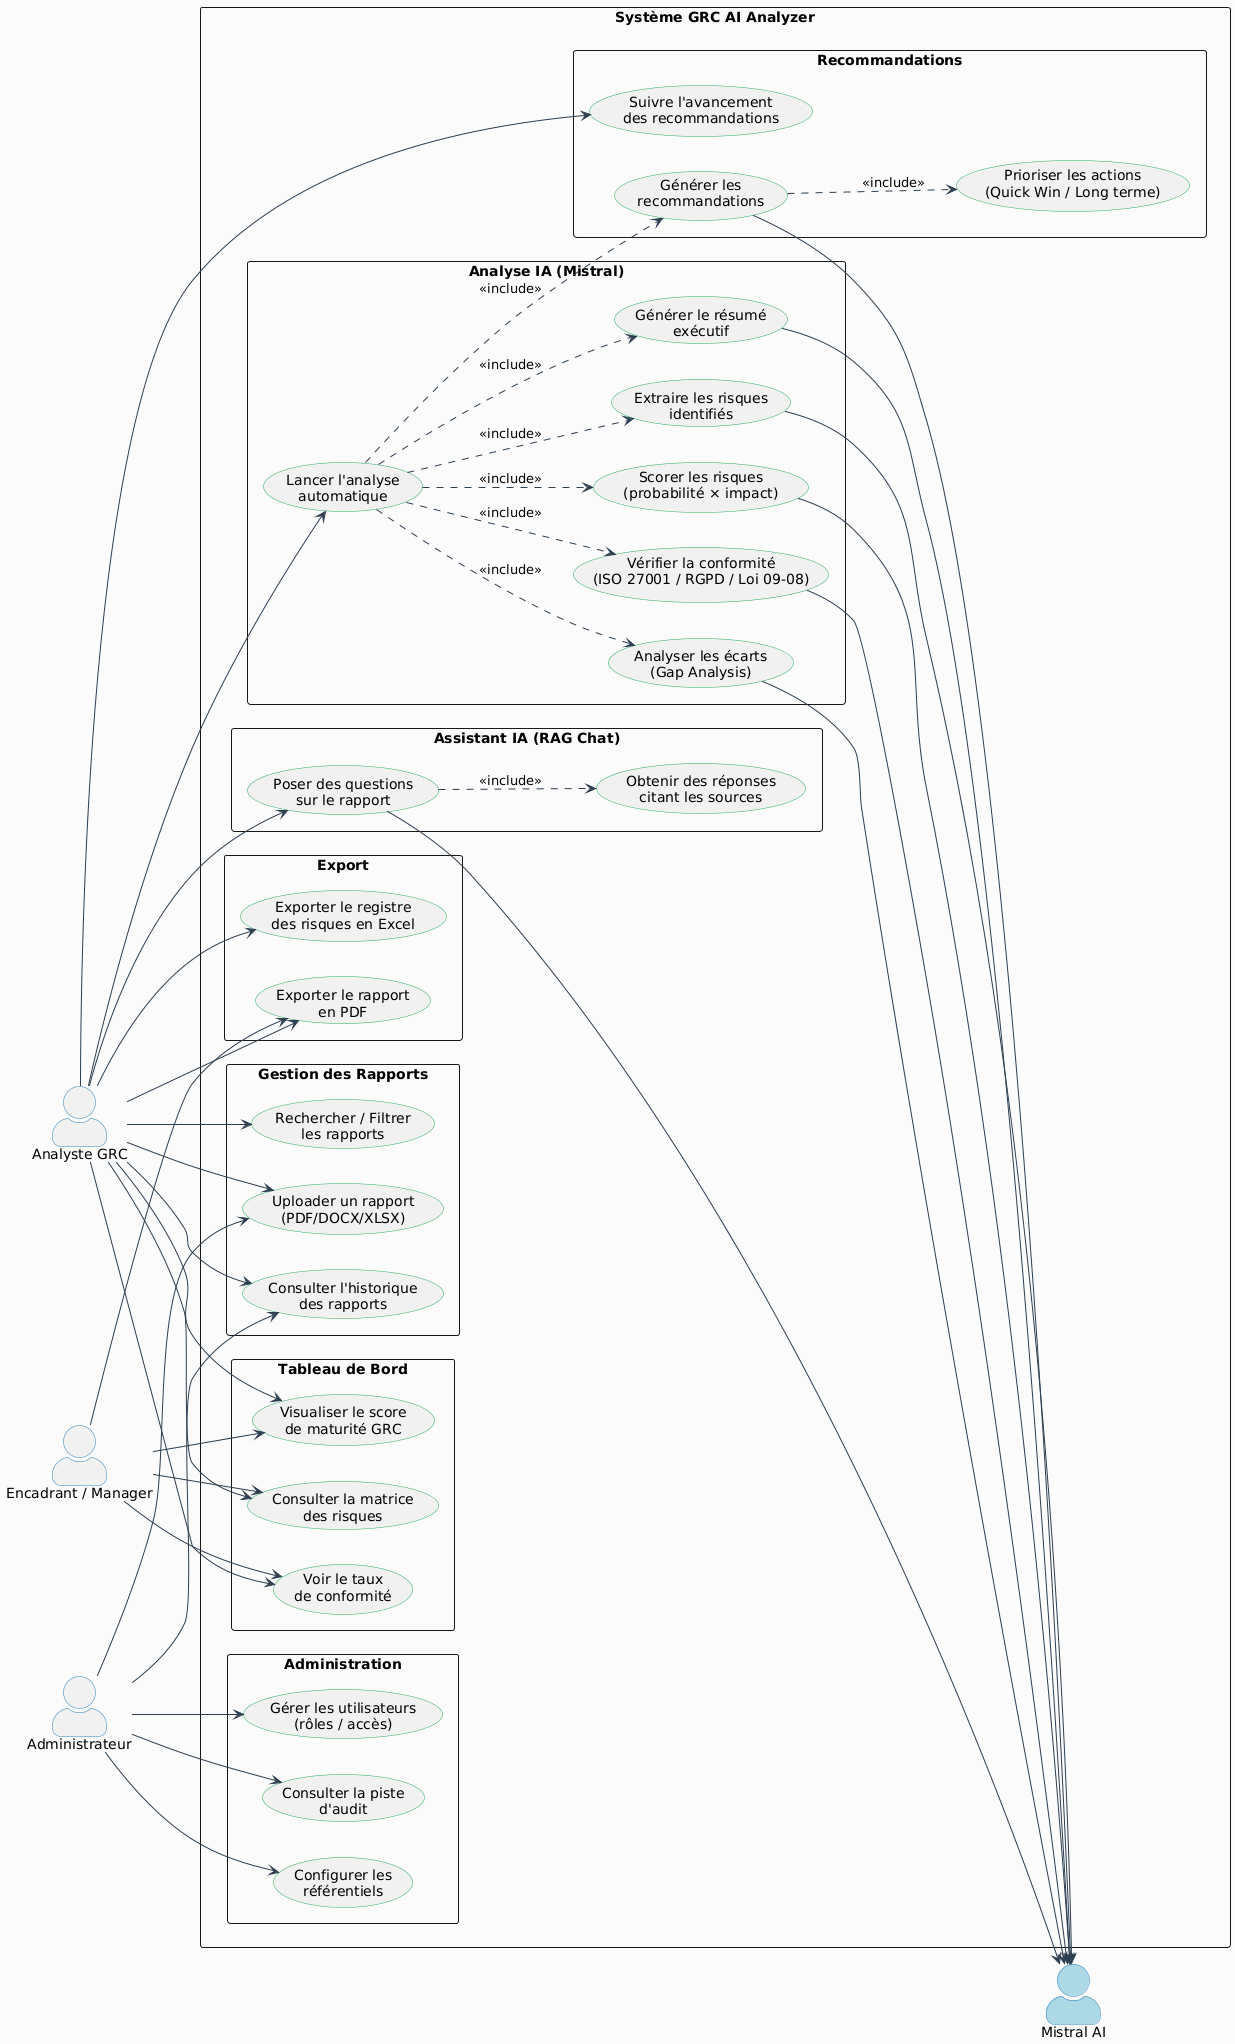
\includegraphics[width=0.92\textwidth]{figures/useC.png}
	\caption{Diagramme des cas d'utilisation — GRC AI Analyzer}
	\label{fig:use_case}
\end{figure}

\subsection{Description des cas d'utilisation principaux}

\subsubsection*{UC-01 : Uploader un rapport}

\begin{tcolorbox}[colback=lightgray!20, colframe=darknavy, title=UC-01 — Uploader un rapport]
	\textbf{Acteur principal :} Analyste GRC \\
	\textbf{Précondition :} L'analyste est authentifié. \\
	\textbf{Scénario nominal :}
	\begin{enumerate}
		\item L'analyste sélectionne un fichier (PDF, DOCX ou XLSX) via l'interface.
		\item Le système valide le format (\texttt{validate\_file\_format}).
		\item Le fichier est sauvegardé sur le serveur sous
		\texttt{uploads/reports/\{uuid\}/\{nom\}}.
		\item Un enregistrement \texttt{Rapport} est créé en base avec le statut
		\textit{en\_attente}.
		\item L'API retourne l'identifiant du rapport (HTTP 201).
	\end{enumerate}
	\textbf{Exception :} Format non supporté → HTTP 400 avec message d'erreur.
\end{tcolorbox}

\subsubsection*{UC-02 : Lancer l'analyse automatique}

\begin{tcolorbox}[colback=lightgray!20, colframe=darknavy, title=UC-02 — Lancer l'analyse automatique]
	\textbf{Acteur principal :} Analyste GRC \\
	\textbf{Acteur secondaire :} Mistral AI \\
	\textbf{Précondition :} Un rapport au statut \textit{en\_attente} existe. \\
	\textbf{Scénario nominal :}
	\begin{enumerate}
		\item L'analyste déclenche l'analyse via
		\texttt{POST /api/v1/analyses/lancer/\{rapport\_id\}}.
		\item Le système crée un enregistrement \texttt{Analyse} (statut
		\textit{en\_cours}) et retourne immédiatement HTTP 202.
		\item En tâche de fond : extraction du texte, chunking, indexation
		ChromaDB, extraction des risques et vérifications de conformité
		(Phase 1 parallèle), puis recommandations et résumé (Phase 2
		parallèle).
		\item L'analyse est marquée \textit{terminé} à la fin du pipeline.
	\end{enumerate}
	\textbf{Cas inclus :} Extraire les risques identifiés ; Scorer les risques ;
	Vérifier la conformité ; Analyser les écarts (Gap Analysis) ;
	Générer le résumé exécutif.
\end{tcolorbox}

\subsubsection*{UC-03 : Poser des questions via le Chat IA}

\begin{tcolorbox}[colback=lightgray!20, colframe=darknavy, title=UC-03 — Poser des questions sur le rapport (RAG Chat)]
	\textbf{Acteur principal :} Analyste GRC \\
	\textbf{Acteur secondaire :} Mistral AI \\
	\textbf{Précondition :} L'analyse est terminée et les chunks ont été indexés. \\
	\textbf{Scénario nominal :}
	\begin{enumerate}
		\item L'analyste saisit une question dans l'onglet Assistant RAG.
		\item Le système encode la question via le modèle sentence-transformer.
		\item ChromaDB retourne les 5 chunks les plus proches par similarité cosinus.
		\item Le système construit le prompt contextuel et interroge Mistral.
		\item La réponse est affichée avec les extraits sources cités.
	\end{enumerate}
	\textbf{Cas inclus :} Obtenir des réponses citant les sources.
\end{tcolorbox}

\subsubsection*{UC-04 : Exporter les livrables}

L'analyste peut exporter deux types de livrables depuis l'interface :
\begin{itemize}
	\item \textbf{Export PDF} — rapport d'analyse complet généré par
	ReportLab, comprenant une page de couverture avec score de maturité,
	un résumé exécutif, un tableau des risques avec badges de sévérité
	colorés, les résultats de conformité par référentiel et le plan de
	recommandations.
	\item \textbf{Export Excel} — registre des risques au format XLSX
	(XlsxWriter) avec quatre onglets structurés et mise en forme
	conditionnelle par sévérité et priorité.
\end{itemize}

\subsubsection*{UC-05 : Suivre l'avancement des recommandations}

L'analyste peut faire progresser le statut de chaque recommandation
via l'interface (bouton de cycle d'état) :
\textit{À\_FAIRE} $\rightarrow$ \textit{EN\_COURS} $\rightarrow$
\textit{CLÔTURÉ}, en appelant
\texttt{PATCH /api/v1/recommandations/\{id\}/statut}.

% ============================================================
\section{Diagramme de Classes}
% ============================================================

\subsection{Vue d'ensemble}

Le diagramme de classes (figure~\ref{fig:class_diagram}) modélise les
entités persistantes du domaine et leurs relations. Il reflète fidèlement
le schéma de base de données PostgreSQL géré par SQLAlchemy (ORM asynchrone)
et versionné via Alembic.

\begin{figure}[H]
	\centering
	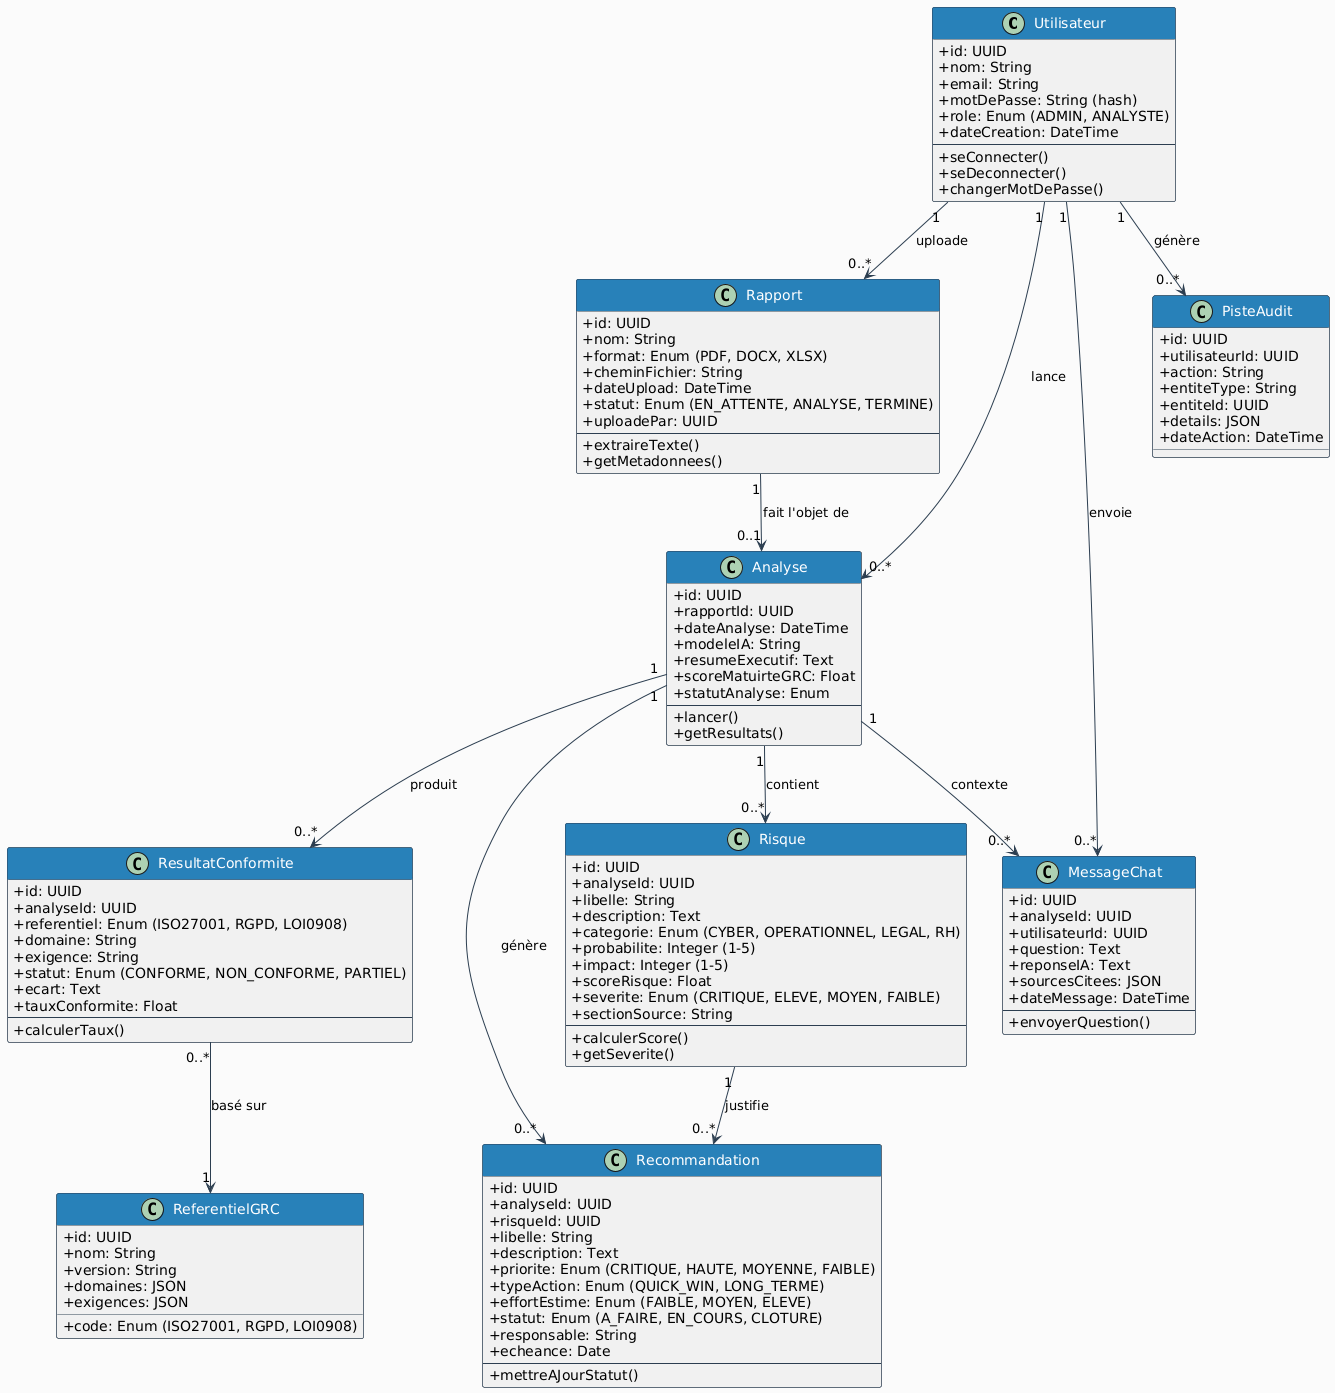
\includegraphics[width=0.95\textwidth]{figures/class.png}
	\caption{Diagramme de classes — modèle du domaine GRC AI Analyzer}
	\label{fig:class_diagram}
\end{figure}

\subsection{Description des classes principales}

\subsubsection*{Utilisateur}

La classe \texttt{Utilisateur} représente les comptes de la plateforme.
Chaque utilisateur possède un identifiant UUID, un nom, un email unique
(indexé), un mot de passe haché (bcrypt), un rôle énuméré
(\texttt{ADMIN} ou \texttt{ANALYSTE}) et une date de création.
Un utilisateur peut uploader plusieurs rapports et déclencher plusieurs
analyses (relations \textit{one-to-many}).

\subsubsection*{Rapport}

La classe \texttt{Rapport} encapsule les métadonnées d'un document soumis
à analyse. Elle stocke le nom du fichier, le format (\texttt{pdf},
\texttt{docx}, \texttt{xlsx}), le chemin de stockage sur disque (chaîne
de type \texttt{reports/\{uuid\}/\{nom\}}), et le statut du cycle de vie
(\textit{en\_attente} → \textit{en\_cours} → \textit{terminé} ou
\textit{erreur}). La suppression d'un rapport entraîne la suppression
en cascade de toutes ses analyses associées
(\texttt{cascade="all, delete-orphan"}).

\subsubsection*{Analyse}

La classe \texttt{Analyse} constitue le cœur du modèle. Elle est liée à
un rapport (many-to-one) et à un utilisateur déclencheur. Elle porte le
résumé exécutif (texte libre), le score de maturité GRC (flottant entre
0 et 100), et le statut de traitement. Elle agrège en composition les
risques, les résultats de conformité et les recommandations.

\subsubsection*{Risque}

La classe \texttt{Risque} représente une menace, vulnérabilité ou écart
identifié par Mistral dans le document. Ses attributs clés sont :
\begin{itemize}
	\item \texttt{libelle} — intitulé du risque (500 caractères max)
	\item \texttt{categorie} — taxonomie en cinq valeurs : CYBER,
	OPERATIONNEL, LEGAL, FINANCIER, RH
	\item \texttt{probabilite} et \texttt{impact} — entiers de 1 à 5
	\item \texttt{score\_risque} — produit probabilité × impact (flottant)
	\item \texttt{severite} — calculée automatiquement selon les seuils
	définis dans \texttt{compute\_severity()}
	\item \texttt{section\_source} — référence à l'identifiant ou à la
	section du document source (ex. : \og{}Finding \#3\fg{},
	\og{}Section A.12\fg{})
\end{itemize}

\subsubsection*{ResultatConformite}

La classe \texttt{ResultatConformite} enregistre l'évaluation d'un domaine
de conformité pour un référentiel donné. Ses attributs principaux sont
le référentiel (\texttt{ISO27001}, \texttt{RGPD}, \texttt{LOI0908}), le
nom du domaine évalué, le statut (\texttt{CONFORME} / \texttt{NON\_CONFORME}
/ \texttt{PARTIEL}), l'écart constaté (texte libre) et le taux de
conformité (flottant). Une analyse peut produire jusqu'à 37 enregistrements
de conformité (14 domaines ISO + 12 RGPD + 11 Loi 09-08).

\subsubsection*{Recommandation}

La classe \texttt{Recommandation} modélise une action corrective générée
par Mistral en réponse à un risque. Elle est liée optionnellement à un
risque (\texttt{risque\_id} nullable), permettant la traçabilité
risque-recommandation. Ses attributs incluent : la priorité (CRITIQUE /
HAUTE / MOYENNE / FAIBLE), le type d'action (QUICK\_WIN ou LONG\_TERME),
l'effort estimé (FAIBLE / MOYEN / ÉLEVÉ) et le statut de traitement
(À\_FAIRE / EN\_COURS / CLÔTURÉ).

\subsubsection*{MessageChat}

La classe \texttt{MessageChat} (présente dans le modèle conceptuel) stocke
l'historique des interactions conversationnelles : la question posée par
l'utilisateur, la réponse générée par Mistral et les sources citées
(tableau JSON des extraits ChromaDB).

\subsubsection*{ReferentielGRC}

La classe \texttt{ReferentielGRC} représente la configuration des cadres
normatifs : ISO 27001, RGPD et Loi 09-08. Elle stocke le code du
référentiel, sa version, et la liste de ses domaines et exigences au
format JSON.

\subsubsection*{PisteAudit}

La classe \texttt{PisteAudit} enregistre les actions réalisées par les
utilisateurs (upload, lancement d'analyse, modification de statut),
permettant à l'administrateur de tracer les opérations sensibles via le
type d'entité, l'identifiant de l'entité concernée et les détails en JSON.

\subsection{Relations entre classes}

Le tableau suivant résume les relations de cardinalité du modèle :

\begin{table}[H]
	\centering
	\caption{Relations entre les classes du domaine}
	\begin{tabularx}{\linewidth}{lllX}
		\toprule
		\textbf{Classe source} & \textbf{Relation} & \textbf{Classe cible} & \textbf{Description} \\
		\midrule
		Utilisateur & 1..* (uploade) & Rapport & Un utilisateur peut soumettre plusieurs rapports \\
		Utilisateur & 1..* (lance) & Analyse & Un utilisateur peut déclencher plusieurs analyses \\
		Rapport & 0..1 (fait l'objet de) & Analyse & Un rapport peut être analysé une fois à la fois \\
		Analyse & 0..* (contient) & Risque & Une analyse produit N risques \\
		Analyse & 0..* (produit) & ResultatConformite & Une analyse produit jusqu'à 37 résultats de conformité \\
		Analyse & 0..* (génère) & Recommandation & Une analyse génère une recommandation par risque \\
		Analyse & 0..* (contexte) & MessageChat & Une analyse peut faire l'objet de N questions RAG \\
		Risque & 0..* (justifie) & Recommandation & Un risque peut être lié à une ou plusieurs recommandations \\
		ResultatConformite & basé sur & ReferentielGRC & Les résultats référencent un cadre normatif \\
		Utilisateur & 0..* (génère) & PisteAudit & Les actions utilisateur alimentent la piste d'audit \\
		\bottomrule
	\end{tabularx}
\end{table}

% ============================================================
\section{Diagramme de Séquence}
% ============================================================

\subsection{Séquence principale : Analyse d'un rapport GRC}

Le diagramme de séquence (figure~\ref{fig:sequence_diagram}) décrit les
interactions chronologiques entre les composants lors de l'opération la
plus complexe du système : le lancement et l'exécution complète d'une
analyse IA.

\begin{figure}[H]
	\centering
	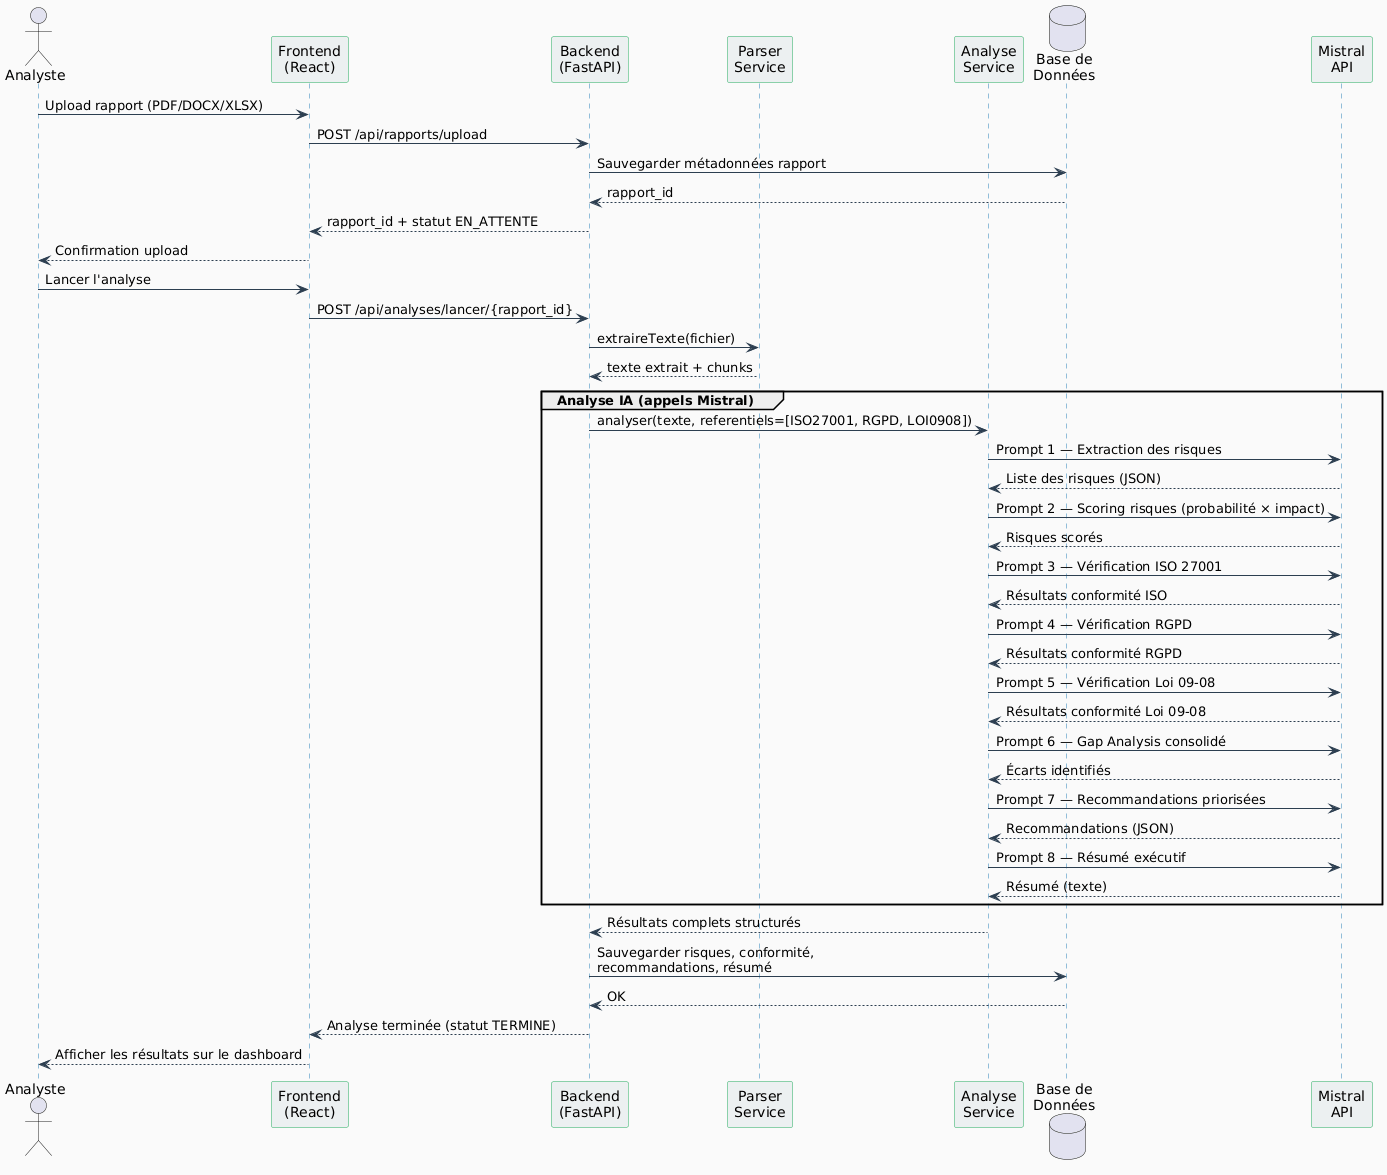
\includegraphics[width=\textwidth]{figures/seq.png}
	\caption{Diagramme de séquence — Analyse d'un rapport GRC}
	\label{fig:sequence_diagram}
\end{figure}

\subsection{Description détaillée des interactions}

Le flux se décompose en deux grandes phases, séparées par une frontière
asynchrone matérialisée par la réponse HTTP 202.

\subsubsection*{Phase synchrone : Upload et déclenchement}

\begin{enumerate}
	\item L'analyste soumet son fichier depuis le frontend React via
	\texttt{POST /api/rapports/upload}. Axios joint le token JWT dans
	l'en-tête de la requête.
	\item Le backend FastAPI valide le format du fichier et délègue au
	\texttt{report\_service} qui sauvegarde le fichier sur disque et
	crée l'enregistrement \texttt{Rapport} en base de données
	(statut : \textit{en\_attente}).
	\item Le frontend reçoit le \texttt{rapport\_id} et affiche une
	confirmation d'upload.
	\item L'analyste déclenche l'analyse via
	\texttt{POST /api/analyses/lancer/\{rapport\_id\}}.
	\item Le backend crée immédiatement l'enregistrement \texttt{Analyse}
	(statut : \textit{en\_cours}), enregistre la tâche de fond via
	\texttt{BackgroundTasks}, et retourne HTTP 202 avec
	l'\texttt{analyse\_id}.
\end{enumerate}

\subsubsection*{Phase asynchrone : Pipeline IA (8 appels Mistral)}

Le service \texttt{analysis\_service.run\_analysis()} s'exécute dans
une session SQLAlchemy dédiée. Il suit le pipeline suivant :

\begin{enumerate}
	\item \textbf{Extraction du texte} — le fichier est lu depuis le disque
	et parsé selon son format. Le texte brut est découpé en chunks.
	
	\item \textbf{Phase 1 — Parallélisation via \texttt{asyncio.gather}} :
	\begin{itemize}
		\item Indexation ChromaDB (embedding des chunks en mémoire)
		\item Prompt 1 → Mistral : extraction exhaustive des risques
		(JSON structuré)
		\item Prompt 2 → Mistral : scoring probabilité × impact des risques
		\item Prompt 3 → Mistral : vérification conformité ISO 27001
		(14 domaines)
		\item Prompt 4 → Mistral : vérification conformité RGPD (12 domaines)
		\item Prompt 5 → Mistral : vérification conformité Loi 09-08
		(11 domaines)
	\end{itemize}
	Les résultats sont validés (sévérités, catégories, doublons) et
	persistés en base de données.
	
	\item \textbf{Gap Analysis consolidée} — à partir des taux de conformité
	calculés, le score de maturité global est déterminé (moyenne des
	trois référentiels).
	
	\item \textbf{Phase 2 — Parallélisation via \texttt{asyncio.gather}} :
	\begin{itemize}
		\item Prompt 7 → Mistral : génération des recommandations priorisées
		(une par risque identifié)
		\item Prompt 8 → Mistral : génération du résumé exécutif
		(350-450 mots, structuré en 6 sections)
	\end{itemize}
	
	\item \textbf{Sauvegarde finale} — l'enregistrement \texttt{Analyse}
	est mis à jour avec le résumé, le score de maturité et le statut
	\textit{terminé}.
\end{enumerate}

\subsubsection*{Phase de consultation}

Le frontend React interroge \texttt{GET /api/analyses/\{id\}} toutes les
4 secondes (polling) jusqu'à obtenir le statut \textit{terminé}.
À ce moment, trois requêtes parallèles (\texttt{Promise.all}) récupèrent
les risques, les résultats de conformité et les recommandations, qui sont
affichés dans les onglets correspondants de la page d'analyse.

% ============================================================
\section{Diagramme d'Activité}
% ============================================================

\subsection{Vue d'ensemble du flux de traitement}

Le diagramme d'activité (figure~\ref{fig:activity_diagram}) modélise le
flux de contrôle complet du système, de l'upload du rapport jusqu'à la
consultation des résultats et l'export des livrables. Il met en évidence
les deux zones de parallélisme (swimlanes horizontaux) correspondant aux
deux phases du pipeline IA.

\begin{figure}[H]
	\centering
	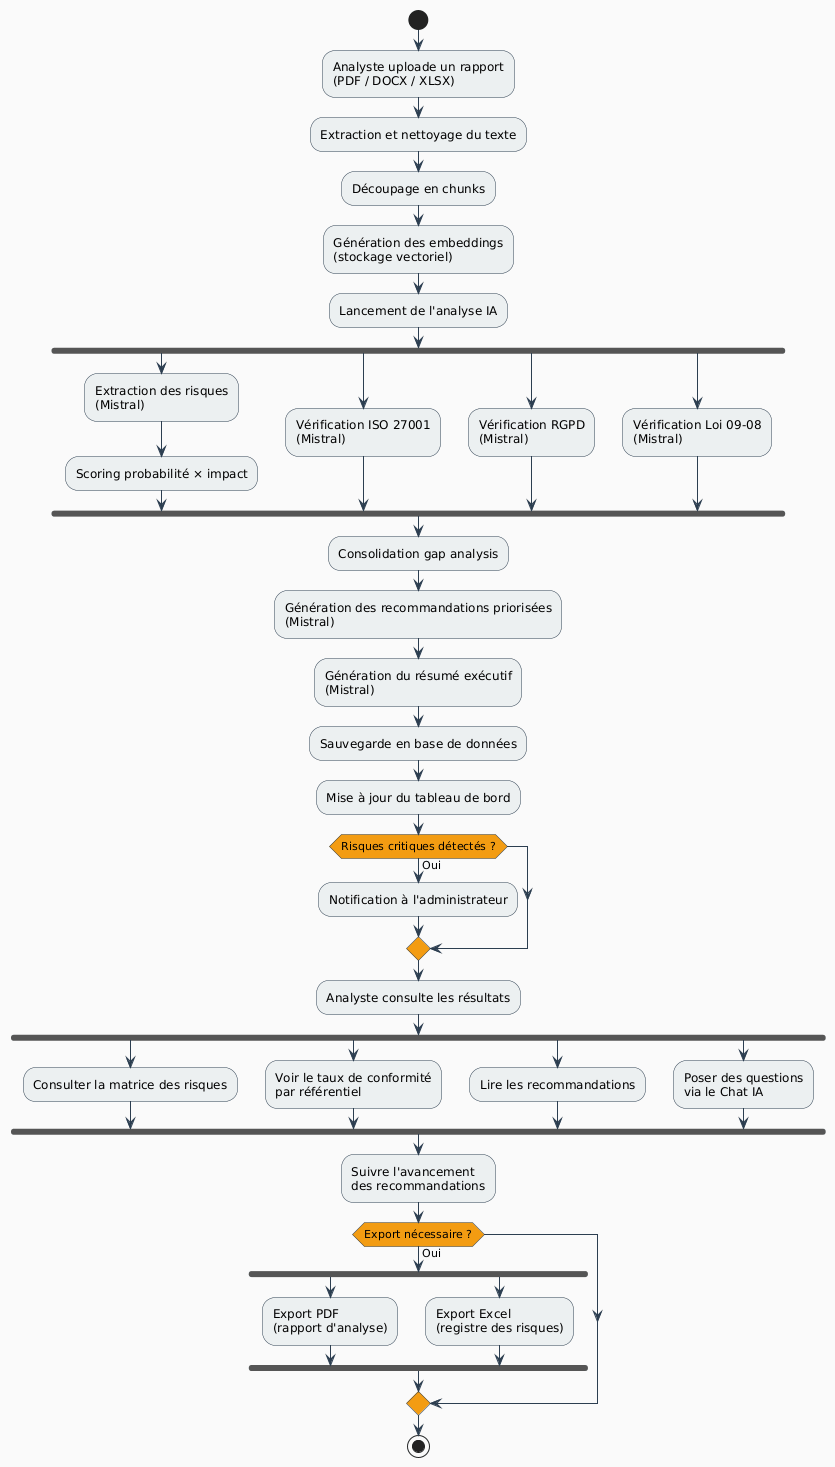
\includegraphics[width=0.85\textwidth]{figures/act.png}
	\caption{Diagramme d'activité — flux de traitement GRC AI Analyzer}
	\label{fig:activity_diagram}
\end{figure}

\subsection{Description des activités}

\subsubsection*{Bloc 1 — Préparation du document}

Les quatre premières activités forment une séquence linéaire :

\begin{enumerate}
	\item \textbf{Upload du rapport} — l'analyste soumet son fichier
	PDF/DOCX/XLSX via l'interface. Le système valide le format,
	sauvegarde le fichier et enregistre les métadonnées.
	\item \textbf{Extraction et nettoyage du texte} — selon le format
	détecté, l'un des trois parsers est appelé (PyMuPDF pour PDF,
	python-docx pour DOCX, openpyxl pour XLSX). Le texte est extrait
	structuré par page, paragraphe ou cellule.
	\item \textbf{Découpage en chunks} — le texte est fragmenté en segments
	de 1 500 caractères avec un chevauchement de 200 caractères assurant
	la continuité sémantique.
	\item \textbf{Génération des embeddings} — chaque chunk est transformé
	en vecteur dense de 384 dimensions par le modèle
	\texttt{paraphrase-multilingual-MiniLM-L12-v2} et indexé dans
	ChromaDB dans une collection nommée
	\texttt{analyse\_\{id\}}.
\end{enumerate}

\subsubsection*{Bloc 2 — Analyse IA parallèle (Phase 1)}

Un nœud de fourche (\textit{fork}) déclenche simultanément quatre
activités parallèles, matérialisant l'utilisation de
\texttt{asyncio.gather} dans le code :

\begin{itemize}
	\item \textbf{Extraction des risques (Mistral)} — appel JSON structuré
	retournant la liste des risques avec libellé, description, catégorie,
	probabilité, impact et référence source.
	\item \textbf{Scoring probabilité × impact} — calcul déterministe du
	score (\textit{score = probabilité × impact}) et classification
	automatique de la sévérité selon les seuils définis.
	\item \textbf{Vérification ISO 27001 (Mistral)} — évaluation des
	14 domaines de l'Annexe A avec statut CONFORME/PARTIEL/NON\_CONFORME
	et taux par domaine.
	\item \textbf{Vérification RGPD (Mistral)} — évaluation des 12 articles
	RGPD pertinents.
	\item \textbf{Vérification Loi 09-08 (Mistral)} — évaluation des
	11 domaines de la loi marocaine de protection des données.
\end{itemize}

Un nœud de jonction (\textit{join}) synchronise les cinq activités
parallèles avant de passer à la consolidation.

\subsubsection*{Bloc 3 — Consolidation et génération (Phase 2)}

\begin{enumerate}
	\item \textbf{Consolidation gap analysis} — les taux de conformité
	sont agrégés, le score de maturité global est calculé.
	\item \textbf{Génération des recommandations priorisées (Mistral)} et
	\textbf{génération du résumé exécutif (Mistral)} s'exécutent en
	parallèle.
	\item \textbf{Sauvegarde en base de données} — tous les objets (risques,
	conformités, recommandations, résumé) sont persistés dans PostgreSQL.
	\item \textbf{Mise à jour du tableau de bord} — le statut de l'analyse
	passe à \textit{terminé}.
\end{enumerate}

\subsubsection*{Décision : Risques critiques détectés ?}

Après la mise à jour du tableau de bord, un nœud de décision vérifie
la présence de risques de sévérité CRITIQUE (score $\geq$ 20). Si oui,
une notification est envoyée à l'administrateur. Dans les deux cas,
l'analyste est redirigé vers la page des résultats.

\subsubsection*{Bloc 4 — Consultation des résultats (parallèle)}

L'analyste dispose de quatre vues accessibles simultanément via les
onglets de l'interface :
\begin{itemize}
	\item \textbf{Matrice des risques} — visualisation Probabilité × Impact
	via \texttt{RiskMatrix} (Recharts).
	\item \textbf{Taux de conformité par référentiel} — radar chart
	via \texttt{ComplianceRadar} (Recharts).
	\item \textbf{Recommandations} — plan d'action priorisé avec gestion
	du cycle de vie.
	\item \textbf{Chat IA} — assistant conversationnel RAG (Mistral +
	ChromaDB).
\end{itemize}

Puis l'analyste peut suivre l'avancement des recommandations au fil
du temps.

\subsubsection*{Décision : Export nécessaire ?}

Si l'analyste souhaite exporter, un nœud de fourche permet de générer
en parallèle le rapport PDF (ReportLab) et/ou le registre Excel
(XlsxWriter), avant de converger vers la fin du flux.

% ============================================================
\section*{Conclusion}
% ============================================================

Ce chapitre a établi les fondements conceptuels de la plateforme GRC AI
Analyzer. L'analyse des besoins a permis d'identifier 24 besoins
fonctionnels répartis en six modules et 13 besoins non fonctionnels
couvrant la performance, la fiabilité, la sécurité et la maintenabilité.
Le diagramme des cas d'utilisation a formalisé les interactions entre les
trois acteurs humains et le modèle Mistral AI. Le diagramme de classes a
modélisé les huit entités persistantes du domaine et leurs relations de
composition et d'association. Le diagramme de séquence a détaillé les
huit appels successifs à l'API Mistral orchestrés en deux phases de
parallélisme. Enfin, le diagramme d'activité a retranscrit le flux complet
du traitement, depuis l'upload jusqu'à l'export des livrables.

Ces artefacts constituent la référence pour le chapitre suivant, qui
présentera l'implémentation concrète de la solution.

% =============================================================================
%  CHAPITRE 3
% =============================================================================
\chapter{Conception technique et choix technologiques}

\begin{tcolorbox}[infobox]
\itshape D\'efinition de l'architecture cible, structuration des couches applicatives, conception du pipeline IA et du moteur RAG, et justification des outils utilis\'es.
\end{tcolorbox}

\section{Introduction}
Apr\`es l'analyse fonctionnelle, ce chapitre introduit la conception technique de la solution.

\section{Vision g\'en\'erale de la solution cible}

L'architecture cible repose sur une s\'eparation nette entre la pr\'esentation (React), l'orchestration et la s\'ecurit\'e (FastAPI), les services IA (Mistral + ChromaDB) et la persistance (PostgreSQL + MinIO).

\begin{figure}[ht]
\centering
\begin{tikzpicture}[node distance=1cm and 1.2cm]
  \tikzstyle{client}=[rectangle,draw=darknavy,thick,fill=lightgray,minimum width=4cm,minimum height=1cm,rounded corners=3pt,align=center]
  \tikzstyle{server}=[rectangle,draw=darknavy,thick,fill=darknavy!15,minimum width=4cm,minimum height=1cm,rounded corners=3pt,align=center]
  \tikzstyle{store}=[cylinder,draw=darknavy,thick,fill=boxgray,minimum width=2cm,minimum height=1.5cm,shape border rotate=90,aspect=0.3,align=center]
  \tikzstyle{ext}=[rectangle,draw=darkgreen,thick,fill=darkgreen!10,minimum width=3cm,minimum height=1cm,rounded corners=3pt,align=center]

  \node[client] (front) {\textbf{React + Vite}\\Frontend SPA};
  \node[server,below=of front] (api) {\textbf{FastAPI Backend}\\API REST asynchrone};

  \node[store,below left=of api,xshift=-0.5cm] (pg) {\textbf{Postgres}\\m\'etadonn\'ees};
  \node[store,below=of api,yshift=-0.3cm] (minio) {\textbf{MinIO}\\fichiers};
  \node[store,below right=of api,xshift=0.5cm] (chroma) {\textbf{ChromaDB}\\vecteurs};

  \node[ext,right=of api] (mistral) {\textbf{Mistral AI}\\(externe)};

  \draw[-{Latex[length=2mm]},thick] (front) -- node[right]{\small HTTPS + JWT} (api);
  \draw[-{Latex[length=2mm]}] (api) -- (pg);
  \draw[-{Latex[length=2mm]}] (api) -- (minio);
  \draw[-{Latex[length=2mm]}] (api) -- (chroma);
  \draw[-{Latex[length=2mm]},dashed] (api) -- node[above]{\small REST} (mistral);
\end{tikzpicture}
\caption{Architecture globale de GRC AI Analyzer}
\label{fig:archi-globale}
\end{figure}

\subsection{Principes directeurs}

\begin{enumerate}[leftmargin=2em,itemsep=4pt]
  \item \textbf{D\'ecouplage frontend/backend.} Le frontend React communique uniquement via une API REST.
  \item \textbf{Asynchronisme natif.} FastAPI avec async/await et asyncio.gather permet d'ex\'ecuter en parall\`ele les appels IA.
  \item \textbf{Pipeline d'analyse en arri\`ere-plan.} L'analyse longue est ex\'ecut\'ee dans un BackgroundTask avec sa propre session asynchrone.
  \item \textbf{S\'erialisation des appels Mistral.} Un asyncio.Semaphore(1) global \'evite les erreurs 429.
  \item \textbf{S\'eparation des stockages.} M\'etadonn\'ees dans PostgreSQL, fichiers dans MinIO, vecteurs dans ChromaDB.
\end{enumerate}

\section{Architecture en couches du backend}

\begin{figure}[ht]
\centering
\begin{tikzpicture}[node distance=0.3cm]
  \tikzstyle{layer}=[rectangle,draw=darknavy,thick,minimum width=11cm,minimum height=0.9cm,rounded corners=2pt,align=center]
  \node[layer,fill=lightgray] (api) {\textbf{Couche API} -- routes FastAPI minces};
  \node[layer,fill=lightgray!70,below=of api] (svc) {\textbf{Couche Services} -- logique m\'etier};
  \node[layer,fill=darknavy!15,below=of svc] (ai) {\textbf{Couche AI} -- prompts, parsers, RAG, embeddings};
  \node[layer,fill=boxgray,below=of ai] (model) {\textbf{Couche Mod\`eles} -- ORM SQLAlchemy};
  \node[layer,fill=boxgray!50,below=of model] (core) {\textbf{Couche Core} -- s\'ecurit\'e, deps, config};
\end{tikzpicture}
\caption{Organisation en couches du backend FastAPI}
\label{fig:layers}
\end{figure}

\section{Pipeline d'analyse asynchrone en deux phases}

Le coeur technique du projet : l'analyse d'un rapport est d\'ecompos\'ee en deux phases parall\`eles successives.

\begin{figure}[ht]
\centering
\begin{tikzpicture}[node distance=0.7cm and 0.6cm]
  \tikzstyle{phase}=[rectangle,draw=darknavy,thick,fill=lightgray,minimum width=2.7cm,minimum height=0.9cm,rounded corners=2pt,align=center,font=\small]
  \tikzstyle{phase2}=[rectangle,draw=darknavy,thick,fill=darknavy!15,minimum width=2.7cm,minimum height=0.9cm,rounded corners=2pt,align=center,font=\small]
  \tikzstyle{startend}=[rectangle,draw=darkgreen,thick,fill=darkgreen!10,minimum width=2cm,minimum height=0.7cm,rounded corners=4pt,align=center,font=\small]

  \node[startend] (start) {Upload};
  \node[phase,below right=of start,xshift=-1.5cm] (p1a) {\textbf{Phase 1}\\Indexation RAG};
  \node[phase,right=of p1a] (p1b) {\textbf{Phase 1}\\Extraction risques};
  \node[phase,right=of p1b] (p1c) {\textbf{Phase 1}\\ISO/RGPD/Loi};
  \node[phase2,below=1cm of p1b] (gather1) {asyncio.gather};
  \node[phase,below left=of gather1,xshift=0.5cm] (p2a) {\textbf{Phase 2}\\Recommandations};
  \node[phase,below right=of gather1,xshift=-0.5cm] (p2b) {\textbf{Phase 2}\\Synth\`ese ex\'ecutive};
  \node[phase2,below=of gather1,yshift=-1.6cm] (gather2) {asyncio.gather};
  \node[startend,below=of gather2] (endn) {Statut = termin\'e};

  \draw[-{Latex[length=2mm]}] (start) -- (p1a);
  \draw[-{Latex[length=2mm]}] (start) -- (p1b);
  \draw[-{Latex[length=2mm]}] (start) -- (p1c);
  \draw[-{Latex[length=2mm]}] (p1a) -- (gather1);
  \draw[-{Latex[length=2mm]}] (p1b) -- (gather1);
  \draw[-{Latex[length=2mm]}] (p1c) -- (gather1);
  \draw[-{Latex[length=2mm]}] (gather1) -- (p2a);
  \draw[-{Latex[length=2mm]}] (gather1) -- (p2b);
  \draw[-{Latex[length=2mm]}] (p2a) -- (gather2);
  \draw[-{Latex[length=2mm]}] (p2b) -- (gather2);
  \draw[-{Latex[length=2mm]}] (gather2) -- (endn);
\end{tikzpicture}
\caption{Pipeline d'analyse en deux phases parall\`eles}
\label{fig:pipeline}
\end{figure}

\section{Mod\`ele RAG}

\begin{figure}[ht]
\centering
\begin{tikzpicture}[node distance=0.7cm and 1cm]
  \tikzstyle{stepbox}=[rectangle,draw=darknavy,thick,fill=lightgray,minimum width=2.7cm,minimum height=0.8cm,rounded corners=2pt,align=center,font=\small]
  \tikzstyle{stepai}=[rectangle,draw=darknavy,thick,fill=darknavy!15,minimum width=2.7cm,minimum height=0.8cm,rounded corners=2pt,align=center,font=\small]

  \node[stepbox] (doc) {Document\\(PDF/DOCX/XLSX)};
  \node[stepbox,right=of doc] (chunk) {Chunking\\1500 / 200};
  \node[stepbox,right=of chunk] (embed) {Embeddings\\MiniLM-L12};
  \node[stepbox,right=of embed] (chroma) {ChromaDB};
  \node[stepai,below=1.2cm of chunk] (query) {Question\\utilisateur};
  \node[stepai,right=of query] (search) {Recherche\\top-k};
  \node[stepai,right=of search] (mistral) {Mistral\\(contexte)};

  \draw[-{Latex[length=2mm]}] (doc) -- (chunk);
  \draw[-{Latex[length=2mm]}] (chunk) -- (embed);
  \draw[-{Latex[length=2mm]}] (embed) -- (chroma);
  \draw[-{Latex[length=2mm]}] (query) -- (search);
  \draw[-{Latex[length=2mm]}] (search) -- (mistral);
  \draw[-{Latex[length=2mm]},dashed] (chroma) -- (search);
\end{tikzpicture}
\caption{Pipeline RAG : indexation et requ\^etage}
\label{fig:rag}
\end{figure}

Le mod\`ele d'embeddings retenu est \texttt{paraphrase-multilingual-MiniLM-L12-v2}, choisi pour ses bonnes performances multilingues et sa taille raisonnable.

\section{Mod\`ele de donn\'ees (PostgreSQL)}

\begin{figure}[ht]
\centering
\begin{tikzpicture}[node distance=1cm and 1.3cm,>={Latex[length=2mm]}]
  \tikzstyle{ent}=[rectangle,draw=darknavy,thick,fill=lightgray,minimum width=2.6cm,minimum height=0.9cm,align=center,font=\small\bfseries]
  \node[ent] (user) {Utilisateur};
  \node[ent,right=of user] (rapport) {Rapport};
  \node[ent,right=of rapport] (analyse) {Analyse};
  \node[ent,below=of analyse,xshift=-2.5cm] (risque) {Risque};
  \node[ent,below=of analyse] (conf) {ResultatConf};
  \node[ent,below=of analyse,xshift=2.5cm] (reco) {Recommandation};

  \draw[->] (user) -- (rapport);
  \draw[->] (rapport) -- (analyse);
  \draw[->] (analyse) -- (risque);
  \draw[->] (analyse) -- (conf);
  \draw[->] (analyse) -- (reco);
  \draw[->,dashed] (risque) -- (reco);
\end{tikzpicture}
\caption{Mod\`ele relationnel simplifi\'e}
\label{fig:erd}
\end{figure}

\paragraph{Calcul de criticit\'e d'un risque.} La s\'ev\'erit\'e d'un risque est d\'efinie par :
$$\text{score} = \text{probabilit\'e} \times \text{impact}, \quad (\text{probabilit\'e}, \text{impact}) \in [1,5]^2$$

avec les seuils : FAIBLE $< 6$, MOYEN $< 12$, \'ELEV\'E $< 20$, CRITIQUE $\geq 20$.

\section{Choix technologiques}

\begin{table}[ht]
\centering
\renewcommand{\arraystretch}{1.3}
\begin{tabular}{|l|l|l|}
\hline
\rowcolor{lightgray}
\textbf{Cat\'egorie} & \textbf{Outil retenu} & \textbf{Justification} \\
\hline
Frontend & React 18 + Vite & \parbox[t]{8cm}{\vspace{2pt}SPA performante, \'ecosyst\`eme riche\vspace{2pt}} \\
\hline
UI Library & Tailwind / shadcn & \parbox[t]{8cm}{\vspace{2pt}Design moderne, customisable\vspace{2pt}} \\
\hline
Charts & Recharts & \parbox[t]{8cm}{\vspace{2pt}Composants React natifs\vspace{2pt}} \\
\hline
\'Etat global & Zustand & \parbox[t]{8cm}{\vspace{2pt}Simple, l\'eger\vspace{2pt}} \\
\hline
HTTP & Axios + interceptor & \parbox[t]{8cm}{\vspace{2pt}Gestion JWT centralis\'ee\vspace{2pt}} \\
\hline
Backend & FastAPI 0.110+ & \parbox[t]{8cm}{\vspace{2pt}Async natif, Pydantic, OpenAPI auto\vspace{2pt}} \\
\hline
ORM & SQLAlchemy 2 + asyncpg & \parbox[t]{8cm}{\vspace{2pt}Async, mature\vspace{2pt}} \\
\hline
Migrations & Alembic & \parbox[t]{8cm}{\vspace{2pt}R\'ef\'erence Python\vspace{2pt}} \\
\hline
LLM & Mistral AI & \parbox[t]{8cm}{\vspace{2pt}Bon rapport qualit\'e/prix, multilingue\vspace{2pt}} \\
\hline
Embeddings & sentence-transformers & \parbox[t]{8cm}{\vspace{2pt}Multilingue, l\'eger\vspace{2pt}} \\
\hline
Vector DB & ChromaDB & \parbox[t]{8cm}{\vspace{2pt}Open-source, Python natif\vspace{2pt}} \\
\hline
Object Store & MinIO & \parbox[t]{8cm}{\vspace{2pt}Compatible S3\vspace{2pt}} \\
\hline
RDBMS & PostgreSQL 15 & \parbox[t]{8cm}{\vspace{2pt}Robustesse, JSONB\vspace{2pt}} \\
\hline
PDF Parser & PyMuPDF & \parbox[t]{8cm}{\vspace{2pt}Rapide, qualit\'e \'elev\'ee\vspace{2pt}} \\
\hline
Auth & JWT + bcrypt & \parbox[t]{8cm}{\vspace{2pt}Standard, stateless\vspace{2pt}} \\
\hline
\end{tabular}
\caption{Synth\`ese des choix techniques}
\label{tab:tech}
\end{table}

\section{Principes de s\'ecurit\'e retenus}
\begin{enumerate}[leftmargin=1.8em,itemsep=2pt]
  \item Hash des mots de passe avec bcrypt (cost~12).
  \item JWT sign\'e HS256, expiration 24h, stock\'e c\^ot\'e client.
  \item Validation stricte des entr\'ees via Pydantic.
  \item Limitation des types de fichiers et taille maximale (50~MB).
  \item Isolation des analyses par utilisateur.
  \item Variables sensibles externalis\'ees dans \texttt{.env}.
\end{enumerate}

\section{Conclusion}
La conception technique repose sur une architecture en couches asynchrone, un pipeline IA parall\'elis\'e et un mod\`ele RAG bas\'e sur des embeddings multilingues.

% =============================================================================
%  CHAPITRE 4 - SPRINT 1
% =============================================================================
\chapter{Sprint 1 : Authentification et gestion des utilisateurs}

\begin{tcolorbox}[infobox]
\itshape Mise en place du socle d'authentification, du contr\^ole d'acc\`es bas\'e sur les r\^oles, et des premiers \'ecrans de connexion / inscription.
\end{tcolorbox}

\section{Introduction}
Ce premier sprint pose le socle de la plateforme : sans authentification fiable, aucune fonctionnalit\'e m\'etier ne peut \^etre expos\'ee de mani\`ere s\'ecuris\'ee.

\section{Objectifs et p\'erim\`etre}
\begin{itemize}[leftmargin=1.5em,itemsep=2pt]
  \item Inscription et connexion s\'ecuris\'ee.
  \item G\'en\'eration et v\'erification de tokens JWT.
  \item Hash bcrypt des mots de passe.
  \item Mod\`ele utilisateur et r\^oles RBAC.
  \item Interceptor Axios pour l'injection automatique du token.
\end{itemize}

\section{Diagramme de s\'equence : connexion}

\begin{figure}[ht]
\centering
\begin{tikzpicture}[node distance=2cm,>={Latex[length=2mm]}]
  \tikzstyle{seqactor}=[rectangle,draw=darknavy,thick,fill=lightgray,minimum width=2cm,minimum height=0.7cm,align=center,font=\small\bfseries]

  \node[seqactor] (u) {Utilisateur};
  \node[seqactor,right=of u] (front) {Frontend};
  \node[seqactor,right=of front] (api) {API};
  \node[seqactor,right=of api] (db) {Postgres};

  \draw[densely dotted] (u.south) -- ++(0,-6);
  \draw[densely dotted] (front.south) -- ++(0,-6);
  \draw[densely dotted] (api.south) -- ++(0,-6);
  \draw[densely dotted] (db.south) -- ++(0,-6);

  \draw[->] ([yshift=-0.5cm]u.south) -- node[above,font=\tiny]{login + password} ([yshift=-0.5cm]front.south);
  \draw[->] ([yshift=-1.5cm]front.south) -- node[above,font=\tiny]{POST /auth/login} ([yshift=-1.5cm]api.south);
  \draw[->] ([yshift=-2.5cm]api.south) -- node[above,font=\tiny]{SELECT user} ([yshift=-2.5cm]db.south);
  \draw[<-] ([yshift=-3.3cm]api.south) -- node[above,font=\tiny]{user row} ([yshift=-3.3cm]db.south);
  \draw[<-] ([yshift=-4.3cm]front.south) -- node[above,font=\tiny]{token + user} ([yshift=-4.3cm]api.south);
  \draw[<-] ([yshift=-5.3cm]u.south) -- node[above,font=\tiny]{redirect dashboard} ([yshift=-5.3cm]front.south);
\end{tikzpicture}
\caption{Diagramme de s\'equence -- Connexion JWT}
\label{fig:seq-login}
\end{figure}

\section{Extrait de code : g\'en\'eration JWT}

\begin{lstlisting}[caption={Service d'authentification},label=lst:auth]
from datetime import datetime, timedelta
from jose import jwt
from passlib.context import CryptContext

pwd_context = CryptContext(schemes=["bcrypt"], deprecated="auto")

def hash_password(password: str) -> str:
    return pwd_context.hash(password)

def verify_password(plain: str, hashed: str) -> bool:
    return pwd_context.verify(plain, hashed)

def create_access_token(data: dict, expires_delta: timedelta = None):
    to_encode = data.copy()
    expire = datetime.utcnow() + (expires_delta or timedelta(hours=24))
    to_encode.update({"exp": expire})
    return jwt.encode(to_encode, settings.SECRET_KEY, algorithm="HS256")
\end{lstlisting}

\section{R\'esultats fonctionnels}

\subsection{Interface de connexion}
L'interface de connexion pr\'esente les champs email et mot de passe avec validation client. En cas d'erreur, un message contextualis\'e est affich\'e.

\subsection{Interface d'inscription}
L'inscription requiert nom complet, email, mot de passe et confirmation. Un compte est cr\'e\'e avec le r\^ole utilisateur par d\'efaut.

\subsection{Politique de mot de passe}
La politique impose : minimum 8 caract\`eres, au moins une majuscule, un chiffre et un caract\`ere sp\'ecial.

\section{Difficult\'es rencontr\'ees}
\begin{table}[ht]
\centering
\renewcommand{\arraystretch}{1.3}
\begin{tabular}{|l|l|}
\hline
\rowcolor{lightgray}
\textbf{Difficult\'e} & \textbf{Solution apport\'ee} \\
\hline
\parbox[t]{6cm}{\vspace{2pt}Persistance du token c\^ot\'e client\vspace{2pt}} & \parbox[t]{8cm}{\vspace{2pt}Stockage localStorage + interceptor Axios pour injection automatique\vspace{2pt}} \\
\hline
\parbox[t]{6cm}{\vspace{2pt}CORS entre Vite (5173) et FastAPI (8000)\vspace{2pt}} & \parbox[t]{8cm}{\vspace{2pt}Configuration explicite de CORSMiddleware\vspace{2pt}} \\
\hline
\parbox[t]{6cm}{\vspace{2pt}Migrations Alembic sur Windows\vspace{2pt}} & \parbox[t]{8cm}{\vspace{2pt}Driver psycopg2 synchrone pour Alembic, asyncpg pour le runtime\vspace{2pt}} \\
\hline
\end{tabular}
\caption{Difficult\'es du Sprint 1 et solutions}
\label{tab:diff-s1}
\end{table}

\section{Bilan du Sprint 1}
Le sprint a permis de poser un socle d'authentification fiable, conforme aux standards (JWT, bcrypt, RBAC).

% =============================================================================
%  CHAPITRE 5 - SPRINT 2
% =============================================================================
\chapter{Sprint 2 : Upload et parsing documentaire}

\begin{tcolorbox}[infobox]
\itshape Mise en place du module d'ingestion documentaire : upload, validation, stockage MinIO et extraction de texte multi-format.
\end{tcolorbox}

\section{Introduction}
Le second sprint adresse l'entr\'ee du pipeline : transformer un fichier h\'et\'erog\`ene en texte exploitable par le LLM.

\section{Objectifs}
\begin{itemize}[leftmargin=1.5em,itemsep=2pt]
  \item Upload multipart de fichiers PDF, DOCX, XLSX (max 50~MB).
  \item D\'eduplication par hash SHA-256.
  \item Stockage dans MinIO (bucket \texttt{grc-reports}).
  \item Extraction texte via PyMuPDF / python-docx / openpyxl.
  \item Cr\'eation d'une entit\'e Rapport en base.
\end{itemize}

\section{Architecture du module}

\begin{figure}[ht]
\centering
\begin{tikzpicture}[node distance=0.8cm and 1.2cm]
  \tikzstyle{ubox}=[rectangle,draw=darknavy,thick,fill=lightgray,minimum width=2.7cm,minimum height=0.9cm,rounded corners=2pt,align=center,font=\small]
  \node[ubox] (upload) {Endpoint\\POST /reports};
  \node[ubox,right=of upload] (validate) {Validation\\(format/taille)};
  \node[ubox,right=of validate] (hash) {Hash SHA-256\\d\'eduplication};
  \node[ubox,below=of hash,fill=darknavy!15] (parser) {Parser\\multi-format};
  \node[ubox,below=of validate,fill=boxgray] (minio) {Stockage\\MinIO};
  \node[ubox,below=of upload,fill=boxgray] (db) {Insertion\\Postgres};
  \draw[-{Latex[length=2mm]}] (upload) -- (validate);
  \draw[-{Latex[length=2mm]}] (validate) -- (hash);
  \draw[-{Latex[length=2mm]}] (hash) -- (parser);
  \draw[-{Latex[length=2mm]}] (validate) -- (minio);
  \draw[-{Latex[length=2mm]}] (parser) -- (db);
  \draw[-{Latex[length=2mm]}] (minio) -- (db);
\end{tikzpicture}
\caption{Pipeline d'ingestion documentaire}
\label{fig:upload-pipeline}
\end{figure}

\section{Strat\'egies d'extraction par format}

\begin{table}[ht]
\centering
\renewcommand{\arraystretch}{1.3}
\begin{tabular}{|l|l|l|}
\hline
\rowcolor{lightgray}
\textbf{Format} & \textbf{Biblioth\`eque} & \textbf{Strat\'egie} \\
\hline
PDF & PyMuPDF (\texttt{fitz}) & \parbox[t]{8cm}{\vspace{2pt}Extraction page-par-page, pr\'eservation de l'ordre\vspace{2pt}} \\
\hline
DOCX & python-docx & \parbox[t]{8cm}{\vspace{2pt}It\'eration sur paragraphes et tableaux\vspace{2pt}} \\
\hline
XLSX & openpyxl & \parbox[t]{8cm}{\vspace{2pt}Lecture de toutes les feuilles\vspace{2pt}} \\
\hline
\end{tabular}
\caption{Strat\'egies d'extraction par format documentaire}
\label{tab:parsers}
\end{table}

\section{Chunking et pr\'eparation pour le RAG}
Le texte extrait est d\'ecoup\'e en chunks de 1500 caract\`eres avec un overlap de 200 caract\`eres, garantissant la continuit\'e s\'emantique entre chunks adjacents.

\begin{lstlisting}[caption={Fonction de chunking},label=lst:chunk]
def chunk_text(text: str, size: int = 1500, overlap: int = 200) -> list:
    chunks, start = [], 0
    while start < len(text):
        end = min(start + size, len(text))
        chunks.append(text[start:end])
        start += size - overlap
    return chunks
\end{lstlisting}

\section{Bilan du Sprint 2}
La plateforme accepte d\'esormais des rapports h\'et\'erog\`enes et les pr\'epare pour l'analyse IA, avec d\'eduplication automatique.

% =============================================================================
%  CHAPITRE 6 - SPRINT 3
% =============================================================================
\chapter{Sprint 3 : Pipeline d'analyse IA}

\begin{tcolorbox}[infobox]
\itshape Coeur du projet : extraction des risques, \'evaluation de la conformit\'e ISO~27001, RGPD et Loi 09-08 par appels parall\`eles \`a Mistral AI, puis g\'en\'eration des recommandations.
\end{tcolorbox}

\section{Introduction}
Ce sprint constitue l'apport diff\'erenciant du projet : la transformation d'un texte non structur\'e en une analyse GRC structur\'ee, exploitable et actionnable.

\section{Architecture du pipeline}

\begin{figure}[ht]
\centering
\begin{tikzpicture}[node distance=0.7cm and 0.8cm]
  \tikzstyle{stepbox}=[rectangle,draw=darknavy,thick,fill=lightgray,minimum width=2.5cm,minimum height=0.8cm,rounded corners=2pt,align=center,font=\small]
  \tikzstyle{aibox}=[rectangle,draw=darknavy,thick,fill=darknavy!15,minimum width=2.5cm,minimum height=0.8cm,rounded corners=2pt,align=center,font=\small]

  \node[stepbox] (start) {D\'ebut analyse};
  \node[aibox,below=of start,xshift=-3.5cm] (rag) {Indexation\\RAG};
  \node[aibox,below=of start,xshift=-1.2cm] (risks) {Extraction\\risques};
  \node[aibox,below=of start,xshift=1.2cm] (iso) {Conformit\'e\\ISO 27001};
  \node[aibox,below=of start,xshift=3.5cm] (rgpd) {Conformit\'e\\RGPD};
  \node[aibox,below=of rag,xshift=2.3cm] (loi) {Conformit\'e\\Loi 09-08};
  \node[stepbox,below=of iso,yshift=-0.6cm,fill=darkgreen!15,draw=darkgreen] (g1) {gather() Phase 1};
  \node[aibox,below=of g1,xshift=-1.5cm] (reco) {Recom-\\mandations};
  \node[aibox,below=of g1,xshift=1.5cm] (synth) {Synth\`ese\\ex\'ecutive};
  \node[stepbox,below=of g1,yshift=-1.5cm,fill=darkgreen!15,draw=darkgreen] (g2) {gather() Phase 2};
  \node[stepbox,below=of g2,fill=darkgreen!30,draw=darkgreen] (endnode) {\textbf{statut = termin\'e}};

  \draw[-{Latex[length=2mm]}] (start) -- (rag);
  \draw[-{Latex[length=2mm]}] (start) -- (risks);
  \draw[-{Latex[length=2mm]}] (start) -- (iso);
  \draw[-{Latex[length=2mm]}] (start) -- (rgpd);
  \draw[-{Latex[length=2mm]}] (start) -- (loi);
  \draw[-{Latex[length=2mm]}] (rag) -- (g1);
  \draw[-{Latex[length=2mm]}] (risks) -- (g1);
  \draw[-{Latex[length=2mm]}] (iso) -- (g1);
  \draw[-{Latex[length=2mm]}] (rgpd) -- (g1);
  \draw[-{Latex[length=2mm]}] (loi) -- (g1);
  \draw[-{Latex[length=2mm]}] (g1) -- (reco);
  \draw[-{Latex[length=2mm]}] (g1) -- (synth);
  \draw[-{Latex[length=2mm]}] (reco) -- (g2);
  \draw[-{Latex[length=2mm]}] (synth) -- (g2);
  \draw[-{Latex[length=2mm]}] (g2) -- (endnode);
\end{tikzpicture}
\caption{Pipeline d'analyse en deux phases parall\`eles}
\label{fig:full-pipeline}
\end{figure}

\section{Prompt engineering}

Pour chaque type d'extraction, un prompt sp\'ecialis\'e est construit. Il comporte trois parties : un r\^ole system, le contexte, et un format JSON strict attendu en sortie.

\begin{lstlisting}[caption={Prompt d'extraction de risques},label=lst:prompt-risque]
def build_risk_prompt(text):
    return [
        {"role": "system", "content": "Tu es un expert GRC..."},
        {"role": "user", "content": f"""
Analyse le rapport et extrait les risques en JSON :
{{
  "risques": [
    {{
      "titre": "...",
      "categorie": "operationnel|financier|technologique|reglementaire",
      "probabilite": 1..5,
      "impact": 1..5
    }}
  ]
}}

Rapport :
{text[:8000]}
"""}
    ]
\end{lstlisting}

\section{S\'erialisation des appels Mistral}

\begin{lstlisting}[caption={S\'emaphore global anti rate-limit},label=lst:semaphore]
import asyncio
from mistralai import Mistral

_semaphore = asyncio.Semaphore(1)
_client = Mistral(api_key=settings.MISTRAL_API_KEY)

async def call_mistral(messages, model="mistral-large-latest"):
    async with _semaphore:
        response = await _client.chat.complete_async(
            model=model, messages=messages
        )
        return response.choices[0].message.content
\end{lstlisting}

\section{R\'esultats}

\subsection{Matrice probabilit\'e/impact des risques}

\begin{figure}[ht]
\centering
\begin{tikzpicture}
\begin{axis}[
  xlabel={Probabilit\'e},
  ylabel={Impact},
  xmin=0,xmax=6,ymin=0,ymax=6,
  xtick={1,2,3,4,5},ytick={1,2,3,4,5},
  width=10cm,height=8cm,
  grid=both,
  scatter/classes={
    a={mark=*,green,mark size=3},
    b={mark=*,orange,mark size=3.5},
    c={mark=*,red,mark size=4}
  }
]
\addplot[scatter,only marks,scatter src=explicit symbolic]
  coordinates {
    (1,2)[a] (2,2)[a] (1,3)[a]
    (3,3)[b] (4,3)[b] (2,4)[b]
    (4,5)[c] (5,4)[c] (5,5)[c]
  };
\end{axis}
\end{tikzpicture}
\caption{Matrice probabilit\'e/impact -- exemple de visualisation des risques}
\label{fig:matrice}
\end{figure}

\subsection{Radar de conformit\'e}
Le radar de conformit\'e affiche, pour chaque r\'ef\'erentiel, le pourcentage de contr\^oles satisfaits, partiellement satisfaits ou non satisfaits.

\section{Bilan du Sprint 3}
Le pipeline IA produit des r\'esultats structur\'es exploitables et r\'eduit le temps d'analyse manuelle de plusieurs jours \`a moins de deux minutes par rapport.

% =============================================================================
%  CHAPITRE 7 - SPRINT 4
% =============================================================================
\chapter{Sprint 4 : RAG et chat conversationnel}

\begin{tcolorbox}[infobox]
\itshape Indexation vectorielle avec ChromaDB et mise en place d'une interface conversationnelle permettant d'interroger le rapport analys\'e en langage naturel.
\end{tcolorbox}

\section{Introduction}
Au-del\`a de l'analyse fig\'ee, l'utilisateur souhaite pouvoir poser des questions ouvertes. Le RAG permet de r\'epondre en mobilisant le contenu original du rapport.

\section{Indexation vectorielle}
\`A la fin de l'analyse, les chunks pr\'epar\'es au Sprint 2 sont vectoris\'es par \texttt{paraphrase-multilingual-MiniLM-L12-v2} et stock\'es dans une collection ChromaDB, garantissant l'isolation par analyse.

\begin{lstlisting}[caption={Indexation ChromaDB},label=lst:rag-index]
def index_chunks(analyse_id, chunks):
    collection = chroma_client.get_or_create_collection(
        f"analyse_{analyse_id}"
    )
    embeddings = embedder.encode(chunks).tolist()
    collection.add(
        ids=[f"chunk_{i}" for i in range(len(chunks))],
        documents=chunks,
        embeddings=embeddings
    )
\end{lstlisting}

\section{Pipeline de question-r\'eponse}

\begin{enumerate}[leftmargin=1.8em,itemsep=2pt]
  \item L'utilisateur saisit une question en langage naturel.
  \item Le backend g\'en\`ere l'embedding de la question.
  \item ChromaDB retourne les $k=5$ chunks les plus similaires.
  \item Un prompt augment\'e est compos\'e (question + extraits cit\'es).
  \item Mistral g\'en\`ere une r\'eponse contextualis\'ee en fran\c{c}ais.
\end{enumerate}

\section{Tol\'erance aux pannes}
Si l'indexation ChromaDB \'echoue, l'analyse principale n'est pas bloqu\'ee : seule la fonctionnalit\'e chat devient indisponible pour cette analyse.

\section{R\'esultats}
L'interface chat s'int\`egre dans la page d'analyse via un panneau lat\'eral. L'utilisateur conserve l'historique de ses questions, et chaque r\'eponse est accompagn\'ee des passages sources cit\'es.

% =============================================================================
%  CHAPITRE 8 - SPRINT 5
% =============================================================================
\chapter{Sprint 5 : Dashboards, exports et supervision}

\begin{tcolorbox}[infobox]
\itshape Visualisation des r\'esultats, exports professionnels (PDF, Excel) et tableau d'administration.
\end{tcolorbox}

\section{Introduction}
Apr\`es la production des donn\'ees d'analyse, ce sprint se concentre sur leur exploitation par l'utilisateur final.

\section{Tableau de bord utilisateur}
La page d'analyse pr\'esente, pour une analyse termin\'ee :
\begin{itemize}[leftmargin=1.5em,itemsep=2pt]
  \item synth\`ese ex\'ecutive ;
  \item matrice probabilit\'e/impact des risques ;
  \item radar de conformit\'e par r\'ef\'erentiel ;
  \item liste paginable des risques avec filtres ;
  \item liste des recommandations associ\'ees.
\end{itemize}

\section{Exports professionnels}
Deux formats sont propos\'es :
\begin{itemize}[leftmargin=1.5em,itemsep=2pt]
  \item \textbf{PDF} (ReportLab) : structur\'e avec couverture, sommaire, sections risques, conformit\'e, recommandations.
  \item \textbf{Excel} (openpyxl) : feuilles Risques, Conformit\'e, Recommandations, avec formules et mise en forme conditionnelle.
\end{itemize}

\section{Polling c\^ot\'e frontend}
La page d'analyse interroge GET /analyses/id toutes les 3 secondes tant que le statut est \texttt{en\_cours}. D\`es que le statut bascule sur \texttt{termine}, le frontend lance en parall\`ele les requ\^etes vers les sous-ressources.

\section{Tableau d'administration}
L'administrateur dispose d'une vue globale : liste des utilisateurs, statistiques, supervision des analyses, et journaux d'audit.

% =============================================================================
%  CONCLUSION GENERALE
% =============================================================================
\chapter*{Conclusion g\'en\'erale et perspectives}
\addcontentsline{toc}{chapter}{Conclusion g\'en\'erale}

\section*{Bilan du projet}
Ce projet de fin d'\'etudes a permis de concevoir, d\'evelopper et d\'eployer une plateforme full-stack d'analyse automatis\'ee des rapports GRC, baptis\'ee \textbf{GRC AI Analyzer}. La solution combine l'efficacit\'e des LLM modernes (Mistral AI), la pertinence du Retrieval Augmented Generation et la robustesse d'une architecture asynchrone, pour transformer un processus manuel en un workflow automatis\'e en quelques minutes.

Les objectifs initiaux ont \'et\'e atteints : la plateforme accepte des documents h\'et\'erog\`enes, extrait automatiquement les risques, \'evalue la conformit\'e par rapport aux trois r\'ef\'erentiels cibles (ISO~27001, RGPD, Loi 09-08), g\'en\`ere des recommandations contextualis\'ees, propose un chat conversationnel et exporte les r\'esultats.

\section*{Apports techniques}
Sur le plan technique, le projet a permis d'approfondir la ma\^itrise de FastAPI en mode asynchrone, l'orchestration parall\`ele, l'int\'egration de LLM externes avec gestion fine du rate limiting, l'utilisation des bases vectorielles et la mise en place d'une architecture en couches claire.

\section*{Apports m\'etier}
Sur le plan m\'etier, GRC AI Analyzer apporte un gain de productivit\'e mesurable, une r\'eduction des biais d'interpr\'etation, une couverture multi-r\'ef\'erentiels coh\'erente, et une capacit\'e d'interrogation conversationnelle in\'edite.

\section*{Perspectives d'\'evolution}
\begin{itemize}[leftmargin=1.5em,itemsep=2pt]
  \item Extension \`a d'autres r\'ef\'erentiels (NIST CSF, PCI-DSS, SOC~2).
  \item Fine-tuning d'un mod\`ele open-source sp\'ecialis\'e.
  \item Module de benchmarking permettant de comparer plusieurs analyses dans le temps.
  \item Workflow d'approbation et de signatures \'electroniques.
  \item Int\'egration avec des outils GRC existants via webhooks.
  \item D\'eploiement Kubernetes avec mise \`a l'\'echelle horizontale.
\end{itemize}

\section*{Apport personnel}
Au-del\`a des comp\'etences techniques, ce projet m'a permis de d\'evelopper une vision globale de la conduite d'un projet logiciel, depuis la compr\'ehension d'un domaine m\'etier complexe jusqu'\`a la livraison d'une solution compl\`ete.

% =============================================================================
%  BIBLIOGRAPHIE
% =============================================================================
\chapter*{Bibliographie et webographie}
\addcontentsline{toc}{chapter}{Bibliographie}

\begin{enumerate}[leftmargin=1.5em,itemsep=2pt]
  \item ISO/IEC 27001:2022 -- Information security management systems -- Requirements.
  \item R\`eglement (UE) 2016/679 du Parlement europ\'een et du Conseil (RGPD).
  \item Loi 09-08 relative \`a la protection des personnes physiques \`a l'\'egard du traitement des donn\'ees \`a caract\`ere personnel, Royaume du Maroc.
  \item Lewis, P. et al., Retrieval-Augmented Generation for Knowledge-Intensive NLP Tasks, NeurIPS, 2020.
  \item Documentation FastAPI -- \url{https://fastapi.tiangolo.com}
  \item Documentation Mistral AI -- \url{https://docs.mistral.ai}
  \item ChromaDB Documentation -- \url{https://docs.trychroma.com}
  \item Reimers, N., Gurevych, I., Sentence-BERT, EMNLP 2019.
  \item Documentation React -- \url{https://react.dev}
  \item Documentation SQLAlchemy 2.0 -- \url{https://docs.sqlalchemy.org}
\end{enumerate}

\end{document}
